\documentclass[a4paper,12pt]{article}
\usepackage[T1]{fontenc}
\usepackage{fullpage,graphicx,psfrag,amsmath,amsfonts}
\usepackage[small,bf]{caption}
\usepackage[utf8]{inputenc}
\usepackage[english]{babel}
\usepackage{lipsum}
\usepackage{url}
\usepackage{bm}
\usepackage{float}
\usepackage{kpfonts}
\usepackage{mathpazo}
\usepackage{physics}
\usepackage{enumitem}
\newtheorem{theorem}{Theorem}
\setitemize{noitemsep,topsep=0pt,parsep=0pt,partopsep=0pt}

\renewcommand*{\a}{\alpha}
\renewcommand*{\t}{\theta}
\renewcommand*{\l}{\ell}
\newcommand*{\T}{^\top}
\newcommand*{\I}{\mathbb{I}}
\newcommand*{\q}{\bm{q}}
\newcommand*{\dotq}{\dot{\q}}
\newcommand*{\de}{\mathop{}\!\mathrm{d}}
\DeclareMathOperator{\sgn}{sgn}

\begin{document}
\author{Filippo Grotto VR460638}

\title{Advanced Control Systems: RPP manipulator}

\maketitle
\tableofcontents

\newpage
\section{Homework List}
\begin{itemize}
    \item HW 1: Direct, inverse, differential kinematics
    \item HW 2: Compute kinetic and potential energy
    \item HW 3: Compute the equations of motion (dynamic model)
    \item HW 4: Compute RNE formulation
    \item HW 5: Compute the dynamic model in the operational space
    \item HW 6: Joint space PD control
    \item HW 7: Joint Space Inverse Dynamics Control
\end{itemize}

\newpage
\section{Kinematics}

\subsection{Direct Kinematics}

\begin{center}
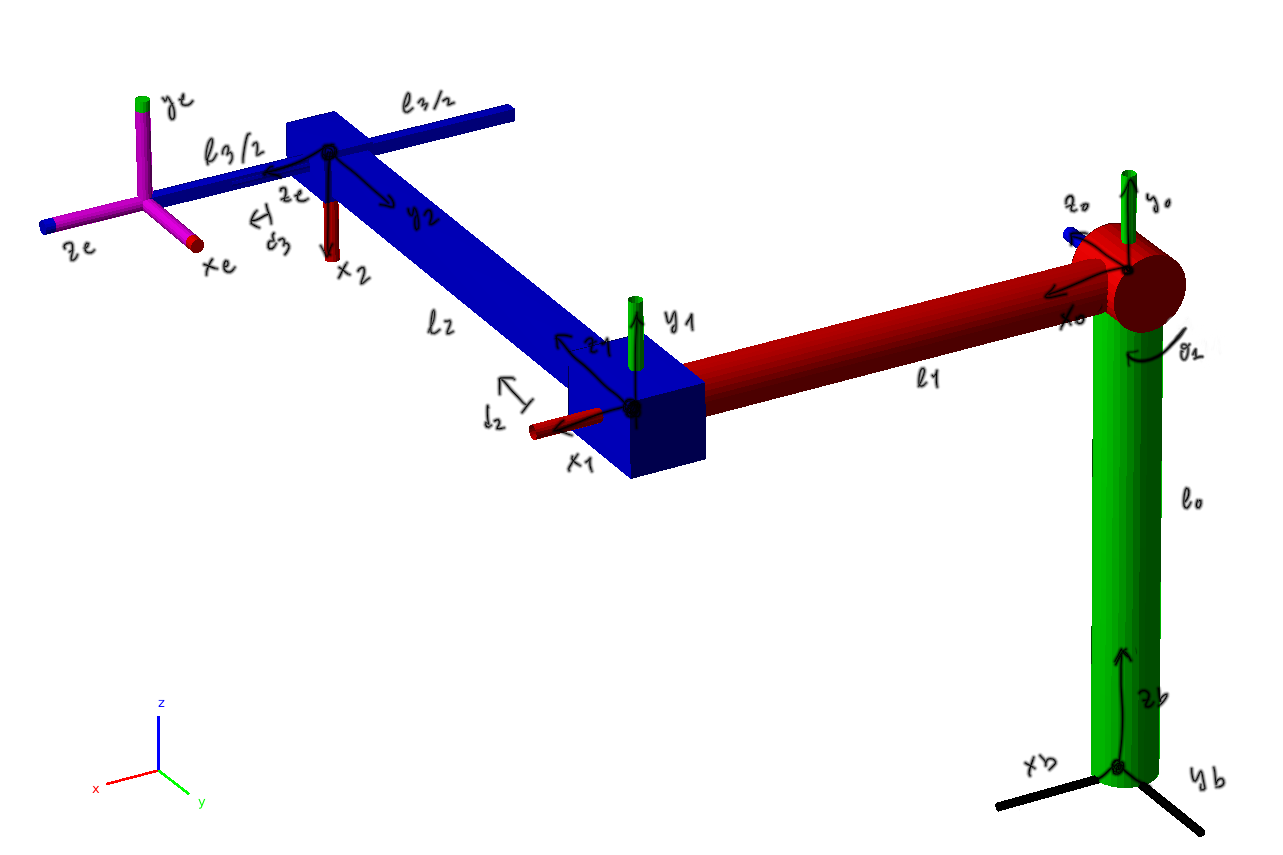
\includegraphics[scale=0.40,trim={10, 10, 10, 10},clip]{images/robot.png}
\end{center}

\noindent Lets define the DH table for our manipulator:

\begin{center}
\begin{tabular}{|c|c|c|c|c|}
    \hline
    $\Sigma_i$ & $d_i$ & $\theta_i$ & $a_i$ & $\alpha_i$ \\ 
    \hline
    $b-0$ & $\l_0$ &    $0$ &    $0$    & $\frac{\pi}{2}$ \\
    $0-1$ &    $0$    & $\t_1$ & $\l_1$ &        $0$ \\
    $1-2$ &    $\l_2+d_2$    & -$\frac{\pi}{2}$ & $0$ &        -$\frac{\pi}{2}$ \\
    $2-3$ &    $\l_3+d_3$ &    $\frac{\pi}{2}$ &    $0$    &        $0$ \\
    $3-e$ &    $0$    &    $0$ &    $0$    &        $0$ \\
    \hline
\end{tabular}
\end{center}

\noindent The homogenous transformation is defined according to the following matrix and calculated for each row of the DH table. By multiplying $H^b_0H^0_1H^1_2H^2_3H^3_e$ we obtain the final transformation
\[
H^{i - 1}_{i}(q_i) = \begin{bmatrix}
    c_{\t_i} &  - s_{\t_i}c_{\a_i} & s_{\t_i}s_{\a_i} & a_i c_{\t_i} \\
    s_{\t_i} & c_{\t_i}c_{\a_i} &  - c_{\t_i}s_{\a_i} & a_i s_{\t_i} \\
        0    &     s_{\a_i}     &     c_{\a_i}     &     d_i     \\
        0    &         0        &         0        &     1        \\
\end{bmatrix}
\]
\[
H^b_0 = \begin{bmatrix}
    1 & 0 & 0 &    0    \\
    0 & 0 &  - 1 &    0    \\
    0 & 1 & 0 & \l_0 \\
    0 & 0 & 0 &    1    \\
\end{bmatrix}
\qquad
\qquad
H^0_1(\t_1) = \begin{bmatrix}
    c_1 &  - s_1 & 0 & \l_1 c_1 \\
    s_1 & c_1 & 0 & \l_1 s_1 \\
        0    &     0    & 1 &        0        \\
        0    &     0    & 0 &        1        \\
\end{bmatrix}
\qquad
H^1_2(d_2) = \begin{bmatrix}
    0 &  0 & 1 & 0 \\
    -1 & 0 & 0 & 0 \\
        0    &    -1    & 0 &        d_2+\l_2       \\
        0    &     0    & 0 &        1        \\
\end{bmatrix}
\]
\[
H^2_3(d_3) = \begin{bmatrix}
    0 & -1 & 0 & 0 \\
    1 & 0 & 0 & 0 \\
    0 & 0 & 1 & d_3 + l_3 \\
    0 & 0 & 0 & 1 \\
\end{bmatrix}
\qquad
H^3_e = \begin{bmatrix}
    1 & 0 & 0 & 0 \\
    0 & 1 & 0 & 0 \\
    0 & 0 & 1 & 0 \\
    0 & 0 & 0 & 1 \\
\end{bmatrix}
\]

\[
H^b_e(\q) = \begin{bmatrix}
    0    &  - s_1 & c_1 & c_1(\l_1+\l_3+d_3)\\
    1   & 0      &  0  &  -\l_2 - d_2 \\
    0    & c_{1} & s_1 & s_1(\l_1+\l_3+d_3) + \l_0 \\
    0    &     0  & 0   &        1       \\
\end{bmatrix}
\qquad
H^0_e(\q) = \begin{bmatrix}
    0    &  - s_1 & c_1 & c_1(\l_1+\l_3+d_3)\\
    0    & c_{1} & s_1 & s_1(\l_1+\l_3+d_3)\\
    -1   & 0      &  0  &  \l_2 + d_2 \\
    0    &     0  & 0   &        1       \\
\end{bmatrix}
\]

\subsection{Inverse Kinematics}
Let's consider the position of ee with respect of the base frame to calculate the value of the joints.
\[
p^b_e = \begin{bmatrix}
    x \\ y \\ z \\
\end{bmatrix}
=
\begin{bmatrix}
    c_1(\l_1+\l_3+d_3)\\
     -\l_2 - d_2 \\
    s_1(\l_1+\l_3+d_3) + \l_0 \\
    1        \\
\end{bmatrix}
\]

It is easy to see that
\[
d_2 = - \l_2 - y \\
\]

\[
\t_1 = \mathop{Atan2}(z-\l_0, x)
\]


For $d_3$ we can apply sum of squares and the result is:
\[
  d_3 = -\l_1 \pm \sqrt{x^2+(z-\l_0)^2} - \l_3  
\]

\section{Differential Kinematics}
\subsection{Geometric Jacobians}
The geometric jacobian is defined as follow with $\q = [\t_1,   d_2,   d_3]^\top$. Note that the matlab robotic toolbox defines the angular velocities above the linear velocities:
\[
\begin{bmatrix}
    \dot{p}_e \\
    \omega_e \\
\end{bmatrix}
 =
\begin{bmatrix}
    \dot{x} \\
    \dot{y} \\
    \dot{z} \\
    \omega_x \\
    \omega_y \\
    \omega_z \\
\end{bmatrix}
 =
\left[
\begin{array}{c|c|c}
    J_{P_1} & J_{P_2} & J_{P_3} \\
    J_{O_1} & J_{O_2} & J_{O_3} \\
\end{array}
\right]
\,
\begin{bmatrix}
    \dot{\t}_1 \\
    \dot{d}_2 \\
    \dot{d}_3 \\
\end{bmatrix}
\]
\begin{align*}
J_{P_1} &= z_0 \times (d^0_e  -  d^0_0) = \begin{bmatrix}
    -s_1(\l_1 + \l_3 + d_3) \\
    0 \\
    c_1(\l_1 + \l_3 + d_3) \\
\end{bmatrix} 
&
J_{O_1} &= z_0 = \begin{bmatrix}0\\-1\\0\end{bmatrix}
\\
J_{P_2} &= z_1 = \begin{bmatrix}
     0 \\
     -1 \\
     0 \\
\end{bmatrix} 
&
J_{O_2} &= \begin{bmatrix}0\\0\\0\end{bmatrix}
\\
J_{P_3} &= z_2 = \begin{bmatrix}
    c_1\\
    0\\
    s_1
\end{bmatrix}
&
J_{O_3} &= \begin{bmatrix}0\\0\\0\end{bmatrix}
\end{align*}
We can finally put all the pieces together and obtain the final geometric jacobian:
\[
J(\q) = 
\begin{bmatrix}
    -s_1(\l_1 + \l_3 + d_3) &  0 & c1 \\
     0 &  -1 & 0 \\
     c_1(\l_1 + \l_3 + d_3) & 0 & s1 \\
    0 & 0 & 0 \\
    -1 & 0 & 0 \\
    0 & 0 & 0 \\
\end{bmatrix}
\qquad
J_0(\q) = 
\begin{bmatrix}
    -s_1(\l_1 + \l_3 + d_3) &  0 & c1 \\
    c_1(\l_1 + \l_3 + d_3) & 0 & s1 \\
     0 &  1 & 0 \\
    0 & 0 & 0 \\
    0 & 0 & 0 \\
    1 & 0 & 0 \\
\end{bmatrix}
\]

\subsection{Analytical Jacobian}
The analytical jacobian can be easily calculated by using partial derivatives of $p^b_e$
\[
p^b_e = \begin{bmatrix}
    x \\ y \\ z \\
\end{bmatrix}
=
\begin{bmatrix}
    c_1(\l_1+\l_3+d_3)\\
     -\l_2 - d_2 \\
    s_1(\l_1+\l_3+d_3) + \l_0 \\
    1        \\
\end{bmatrix}
\]

\noindent Finally we end up with the analytical jacobian
\[
Ja(\q) = 
\begin{bmatrix}
    -s_1(\l_1 + \l_3 + d_3) &  0 & c1 \\
     0 &  -1 & 0 \\
     c_1(\l_1 + \l_3 + d_3) & 0 & s1 \\
    1 & 0 & 0 \\
    0 & 0 & 0 \\
    0 & 0 & 0 \\
\end{bmatrix}
\qquad
Ja_0(\q) = 
\begin{bmatrix}
    -s_1(\l_1 + \l_3 + d_3) &  0 & c1 \\
    c_1(\l_1 + \l_3 + d_3) & 0 & s1 \\
     0 &  1 & 0 \\
    1 & 0 & 0 \\
    0 & 0 & 0 \\
    0 & 0 & 0 \\
\end{bmatrix}
\]

\noindent Another possibility is to use the relation between the geometric and analytical jacobian as follow using ZYZ:

\[
\omega_e = T(\phi_e)\dot{\phi}_e
\qquad
T(\phi_e) = \begin{bmatrix}
    0 & -s_\varphi & c_\varphi s_\theta \\
    0 &  c_\varphi & s_\varphi s_\theta \\
    1 &          0 &           c_\theta \\
\end{bmatrix}
\]

\[
J(\q) = T_A(\phi_e) J_A(\q)
\]
\[
T_A(\phi_e) = \begin{bmatrix}
    \I_3 & \emptyset_3 \\ 
\emptyset_3 &     T(\phi_e) \\
\end{bmatrix}
\]

\section{Lagrangian formulation}
Let's calculate $p_{\l_i}$ of the center of mass wrt of $\Sigma_0$. To get them let's calculate $p^i_{\l_i}$ of the center of mass wrt of $\Sigma_i$
\[
p_{\l_1}^{1} = \begin{bmatrix}  - \frac{\l_1}{2} \\ 0 \\ 0 \end{bmatrix}
\qquad
\qquad
p_{\l_2}^{2} = \begin{bmatrix} 0 \\ \frac{\l_2}{2} \\ 0 \end{bmatrix}
\qquad
\qquad
p_{\l_3}^{3} = \begin{bmatrix} 0 \\ 0 \\  - \frac{\l_3}{2} \end{bmatrix}
\]
we can express the homogenous wrt of $\Sigma_0$ using the following formula: 
\[
p_{\l_i} = R^0_i p_{\l_i}^{i}  +  d^0_i
\] 

\subsection{Potential Energy}
The potential energy is calculated according to the formula:
\[
    U_i = -m_{l_i}g_0^{T}p_{l_i}
    \qquad
    g_0 = \begin{bmatrix}
        0\\ -g \\ 0
    \end{bmatrix}
\]
\noindent The total potential energy is the sum of the 3 contributions $U_1$ $U_2$ and $U_3$. The total expression is reported and was calculated using the MATLAB symbolic toolbox w.r.t of frame 0 ($l_{i}$ is the length of i-th link and $m_i$ is the mass)
\[
    U = \frac{gsin(\theta_1)(l_{1}m_1 + 2l_{1}m_2 + 2l_{1}m_3 + l_{3}m_3 + 2d_3m_3)}{2}  
\]

\subsection{Kinetic Energy}
The kinetic energy is calculated using the following formula:
\[
\mathcal{T}(\q,\dotq) = \frac{1}{2}\dotq\T B(\q) \dotq
\]

\[
B(\q) = \sum_{i=1}^{n} B_i(\q)
      = \sum_{i=1}^{n} m_{\l_i} \bigl({J^{\l_i}_{P}}\T J^{\l_i}_{P}\bigr)
       +  \bigl({R_i^0}\T J^{\l_i}_{O}\bigr)\T I_{\l_i}^{i} \bigl({R_i^0}\T J^{\l_i}_{O}\bigr)
\]

\noindent It is necessary to calculate the inertia tensors $I_{\l_i}^{i}$ and the partial jacobians $J^{\l_i}_{P}$ and $J^{\l_i}_{O}$. We will use the steiner theorem because all frames $\Sigma_i$ are translated of $p_{\l_i}^{i}$ w.r.t. of the center of mass (i.e inertia tensor w.r.t. of the axis of the joint that the
link is attached).
\[
    I_{\l_1}^{1} = I_{\l_1}^{C_1} + m_{\l_1}S^{T}(r)S(r) = I_{\l_1}^{C_1}  +  m_{\l_1}\bigl(r\T r \I_{3,3}  -  r r\T\bigr) 
\]
For the inertia tensors we can use the following formulas for the cylindrical and prismatic links considering that the prismatic links have a square base.
\[
    I^C_{cylinder} = \frac{1}{2}\begin{bmatrix}
        m(a^2+b^2) & 0 &0 \\
        0 &m(3(a^2+b^2)+h^2)& 0 \\
        0& 0& m(3(a^2+b^2)+h^2)
    \end{bmatrix}
\]

\[
    I^C_{prismatic} = \frac{1}{12}\begin{bmatrix}
        m(b^2+c^2) & 0 &0 \\
        0 &m(a^2+c^2)& 0 \\
        0& 0& m(a^2+b^2)
    \end{bmatrix}
\]

\bigskip
\noindent Finally we need to compute the partial jacobians in order to calculate velocity of intermediate links.

\[
    J^{\l_i}_{P_j} = \begin{cases}
       z_{j-1} & \text{prismatic joint} \\
       z_{j-1} \times (p_{l_i}- p_{j-1}) & \text{revolute joint} 
      \end{cases}
    \qquad
    J^{\l_i}_{O_j} = \begin{cases}
    0 & \text{prismatic joint} \\
    z_{j-1} & \text{revolute joint} 
    \end{cases}
\]

\noindent In our case the computer partial jacobians are:

\[
    J^{\l_1}_{P} = \begin{bmatrix}
        -\l_1sin(\theta_1)/2 & 0 & 0 \\
 \l_1cos(\theta_1)/2 &0 &0 \\
               0 &0 &0
    \end{bmatrix}
    \qquad
    J^{\l_2}_{P} = \begin{bmatrix}
        - \l_1sin(\theta_1) &0 &0\\
\l_1cos(\theta_1) & 0 &0\\
                            0& 1& 0;
    \end{bmatrix}
\]
\[
    J^{\l_3}_{P} = \begin{bmatrix}
        -sin(\theta_1)(\l_1 + \l_3/2 + d_3) &0 & cos(\theta_1)\\
 cos(\theta_1)(\l_1 + \l_3/2 + d_3) &0 &sin(\theta_1)\\
                          0 &1 &      0
    \end{bmatrix}
    \qquad
    J^{\l_1}_{O} = J^{\l_2}_{O} = J^{\l_3}_{O} =\begin{bmatrix}
        0 &0 &0\\ 0& 0 &0\\ 1& 0& 0
    \end{bmatrix}
\]

\[
  B(\textbf{q}) = B_1(\textbf{q}) + B_2(\textbf{q}) +B_3(\textbf{q}) 
\]

\noindent Finally we can recover the kinetic energy using the calculated $B(\textbf{q})$ and $ \dot{\textbf{q}}$. In order to verify the following properties has been checked: 
\bigskip
\begin{itemize}
    \item $B(\q) = B(\q)^\top$ symmetric
    \item $B(\q) \succ 0$ positive definite
    \item $T(\q, \dotq) = 0$ if and only if $ \dotq = 0$
    \item $T(\q, \dotq) \geq 0$
\end{itemize}

\subsection{Dynamic Model of the manipulator}
The aim is to find an expression that describes the dynamic model of the manipulator:
\[
    B(q)\ddot{q} + C(q, \dot{q})\dot{q} + g(q) = \tau
\]

\noindent The matrix $B(q)$ was previously calculated as a sum of the contributions of each link and $g(q)$ can be easily derived by differentiating $U$ by the generalized positions $q = [\theta_1,d_2, d_3]$. In order to recover $C(q,\dot{q})$ some additional steps are required and described as follows:
\begin{equation}
    \begin{aligned}
        \sum_{j=1}^{n} c_{ij}(\q, \dotq)\dot{q_j}  &= \sum_{j=1}^{n}\sum_{k=1}^{n} \frac{1}{2} (\pdv{b_{ij}}{q_k}+\pdv{b_{ik}}{q_j}-\pdv{b_{jk}}{q_i})\dot{q_k}\dot{q_j} \\
         &= \sum_{j=1}^{n}\sum_{k=1}^{n} c_{ijk}\dot{q_k}\dot{q_j} \\
         &= \sum_{j=1}^{n} c_{ij}\dot{q_j}
    \end{aligned}
\end{equation}

\noindent A generalized formulation for the dynamic model of the manipulator is
\[
    B(q)\ddot{q} + C(q, \dot{q})\dot{q} + F_v\dot{q} + F_ssign(\dot{q}) + g(q) = \tau - J^{T}(q)h_e  
\]
\subsection{Recursive Newton Euler}
The recursive newton euler has been implemented for the RPP robot. The calculations are lengthy and are not reported here. The results have been compared with the lagrangian model and using the following facts:
\bigskip
\[
    \tau_{d} = NE(q,\dot{q}, \ddot{q}, g_{0})
\]
\noindent Gravity term
\[
    g(q) = NE(q,0,0,g_0)
\]
Centrifugal and coriolis term
\[
    C(q,\dot{q})\dot{q} = NE(q,\dot{q},0,0)
\]
Inertial matrix
\[
    B_i(q) = NE(q,0,e_i,0) \qquad e_i = \text{i-th element equal to 1}
\]
Generalized momentum
\[
    B(q)\dot{q} = NE(q,0,\dot{q},0)
\]
\subsection{Operational space dynamic model}
The operational space dynamic model is defined using the following relations:
\[
    \begin{cases}
    B_{A}(x) = J_{A}^{-1}BJ_A^{-1} \\
    C_{A}(x)\dot{x} = J_{A}^{-1}C\dot{q} - B_{A}\dot{J_{A}}\dot{q} \\
    g_{A}(x) = J_{A}^{-1}g \\
    u = T_{A}^T(x) h \\
    u_e = T_{A}^T(x)h_{e}
    \end{cases}
\]
Under the assumptions that $B_{A}$ is nonsingular $J_{A}$ full rank.

\newpage 
\section{Control architectures}
\subsection{Joint Space PD Control with Gravity Compensation}

The joint space PD Control with gravity compensation was implemented using an S-function to define the manipulator dynamics. In fact the symbolic B,C and G matrixes were used in this context. The values for $Kp$ and $Kd$ has been properly selected for our robot. In Fig \ref{fig:gravity_comp} a plot of the positions with respect of the desired positions are reported as well as the related $tau$ applied to each of the three joints.
\begin{figure}[H]
    \begin{center}
        \hspace*{-4.5cm}
        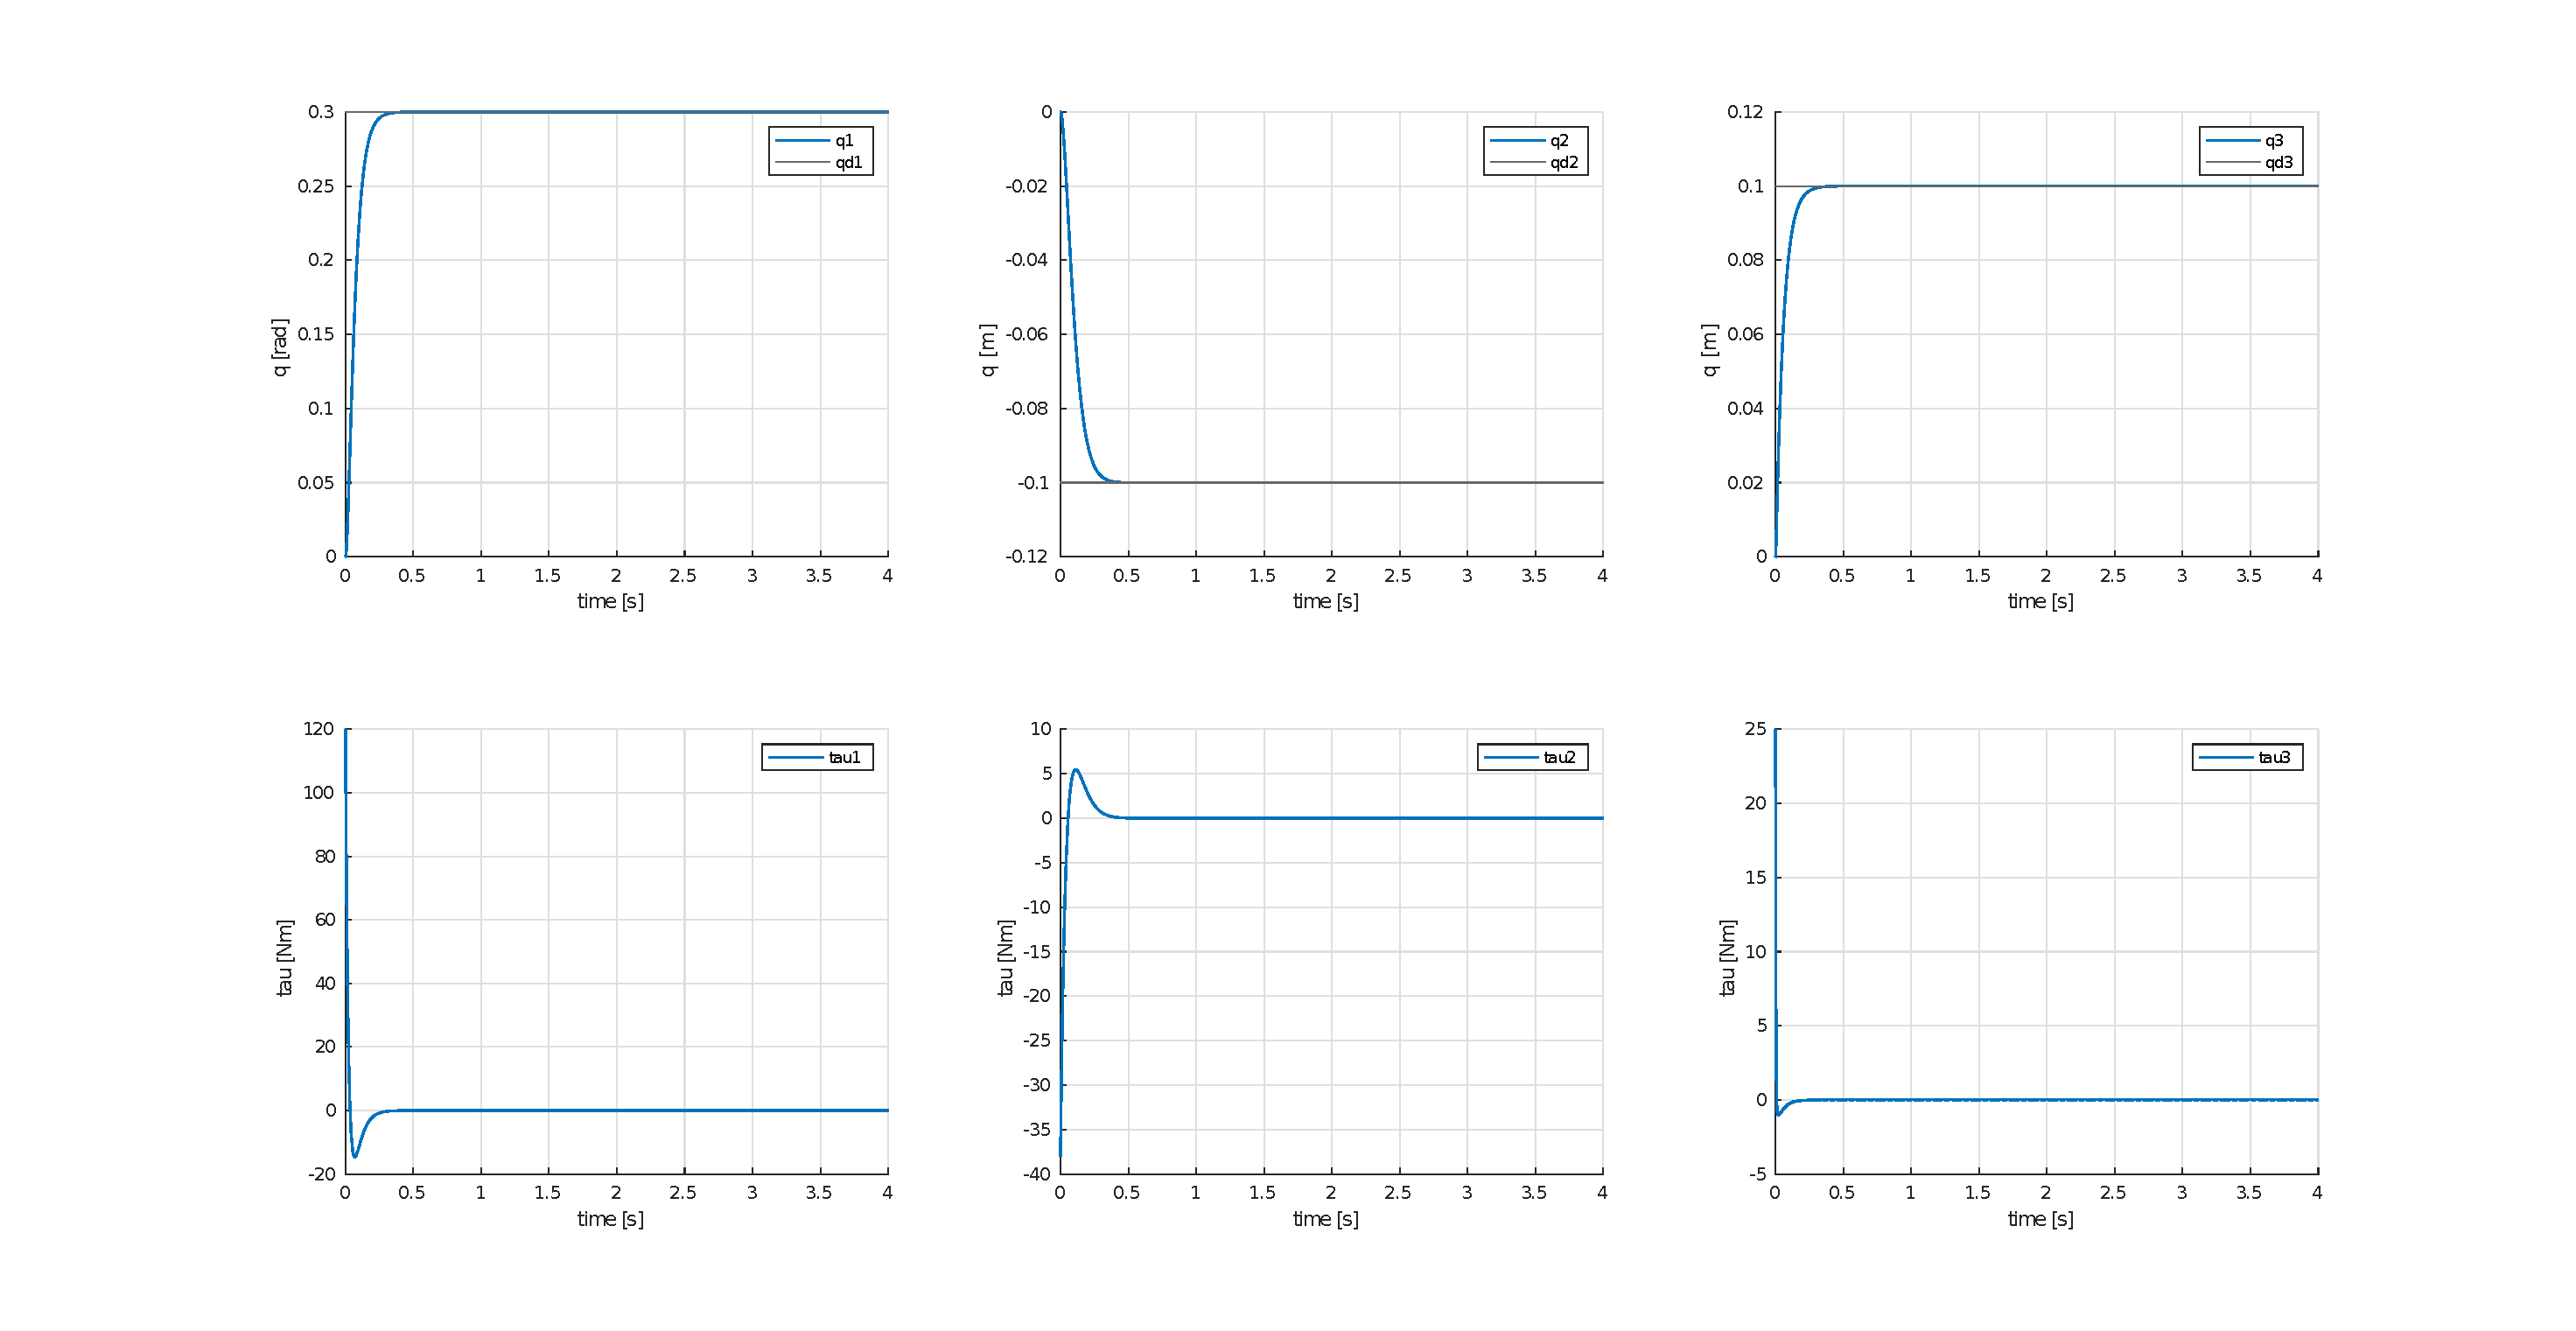
\includegraphics[scale=0.5]{images/gravity_comp.eps}
    \end{center}
    \caption{Joint Space PD Control with Gravity Compensation}
    \label{fig:gravity_comp}
\end{figure}

It is reasonable to tune the 3 joints to get the same time for tracking or at least try to be at the same time. As it is visible from Fig \ref{fig:gravity_comp} we have to find a compromise between performances and the $tau$ required.

\newpage
\subsubsection{Without gravity compensation}
Let's try without the gravity compensation, in Fig \ref{fig:gravity_comp_no_gravity} it's visible that we have an offset in steady-state where the gravity plays a role, in the RPP robot it's the first joint, which is clearly visible, and on the third joint depending on the configuration (in this case the effect is really limited to to the configuration).
\begin{figure}[H]
    \begin{center}
        \hspace*{-4.5cm}
        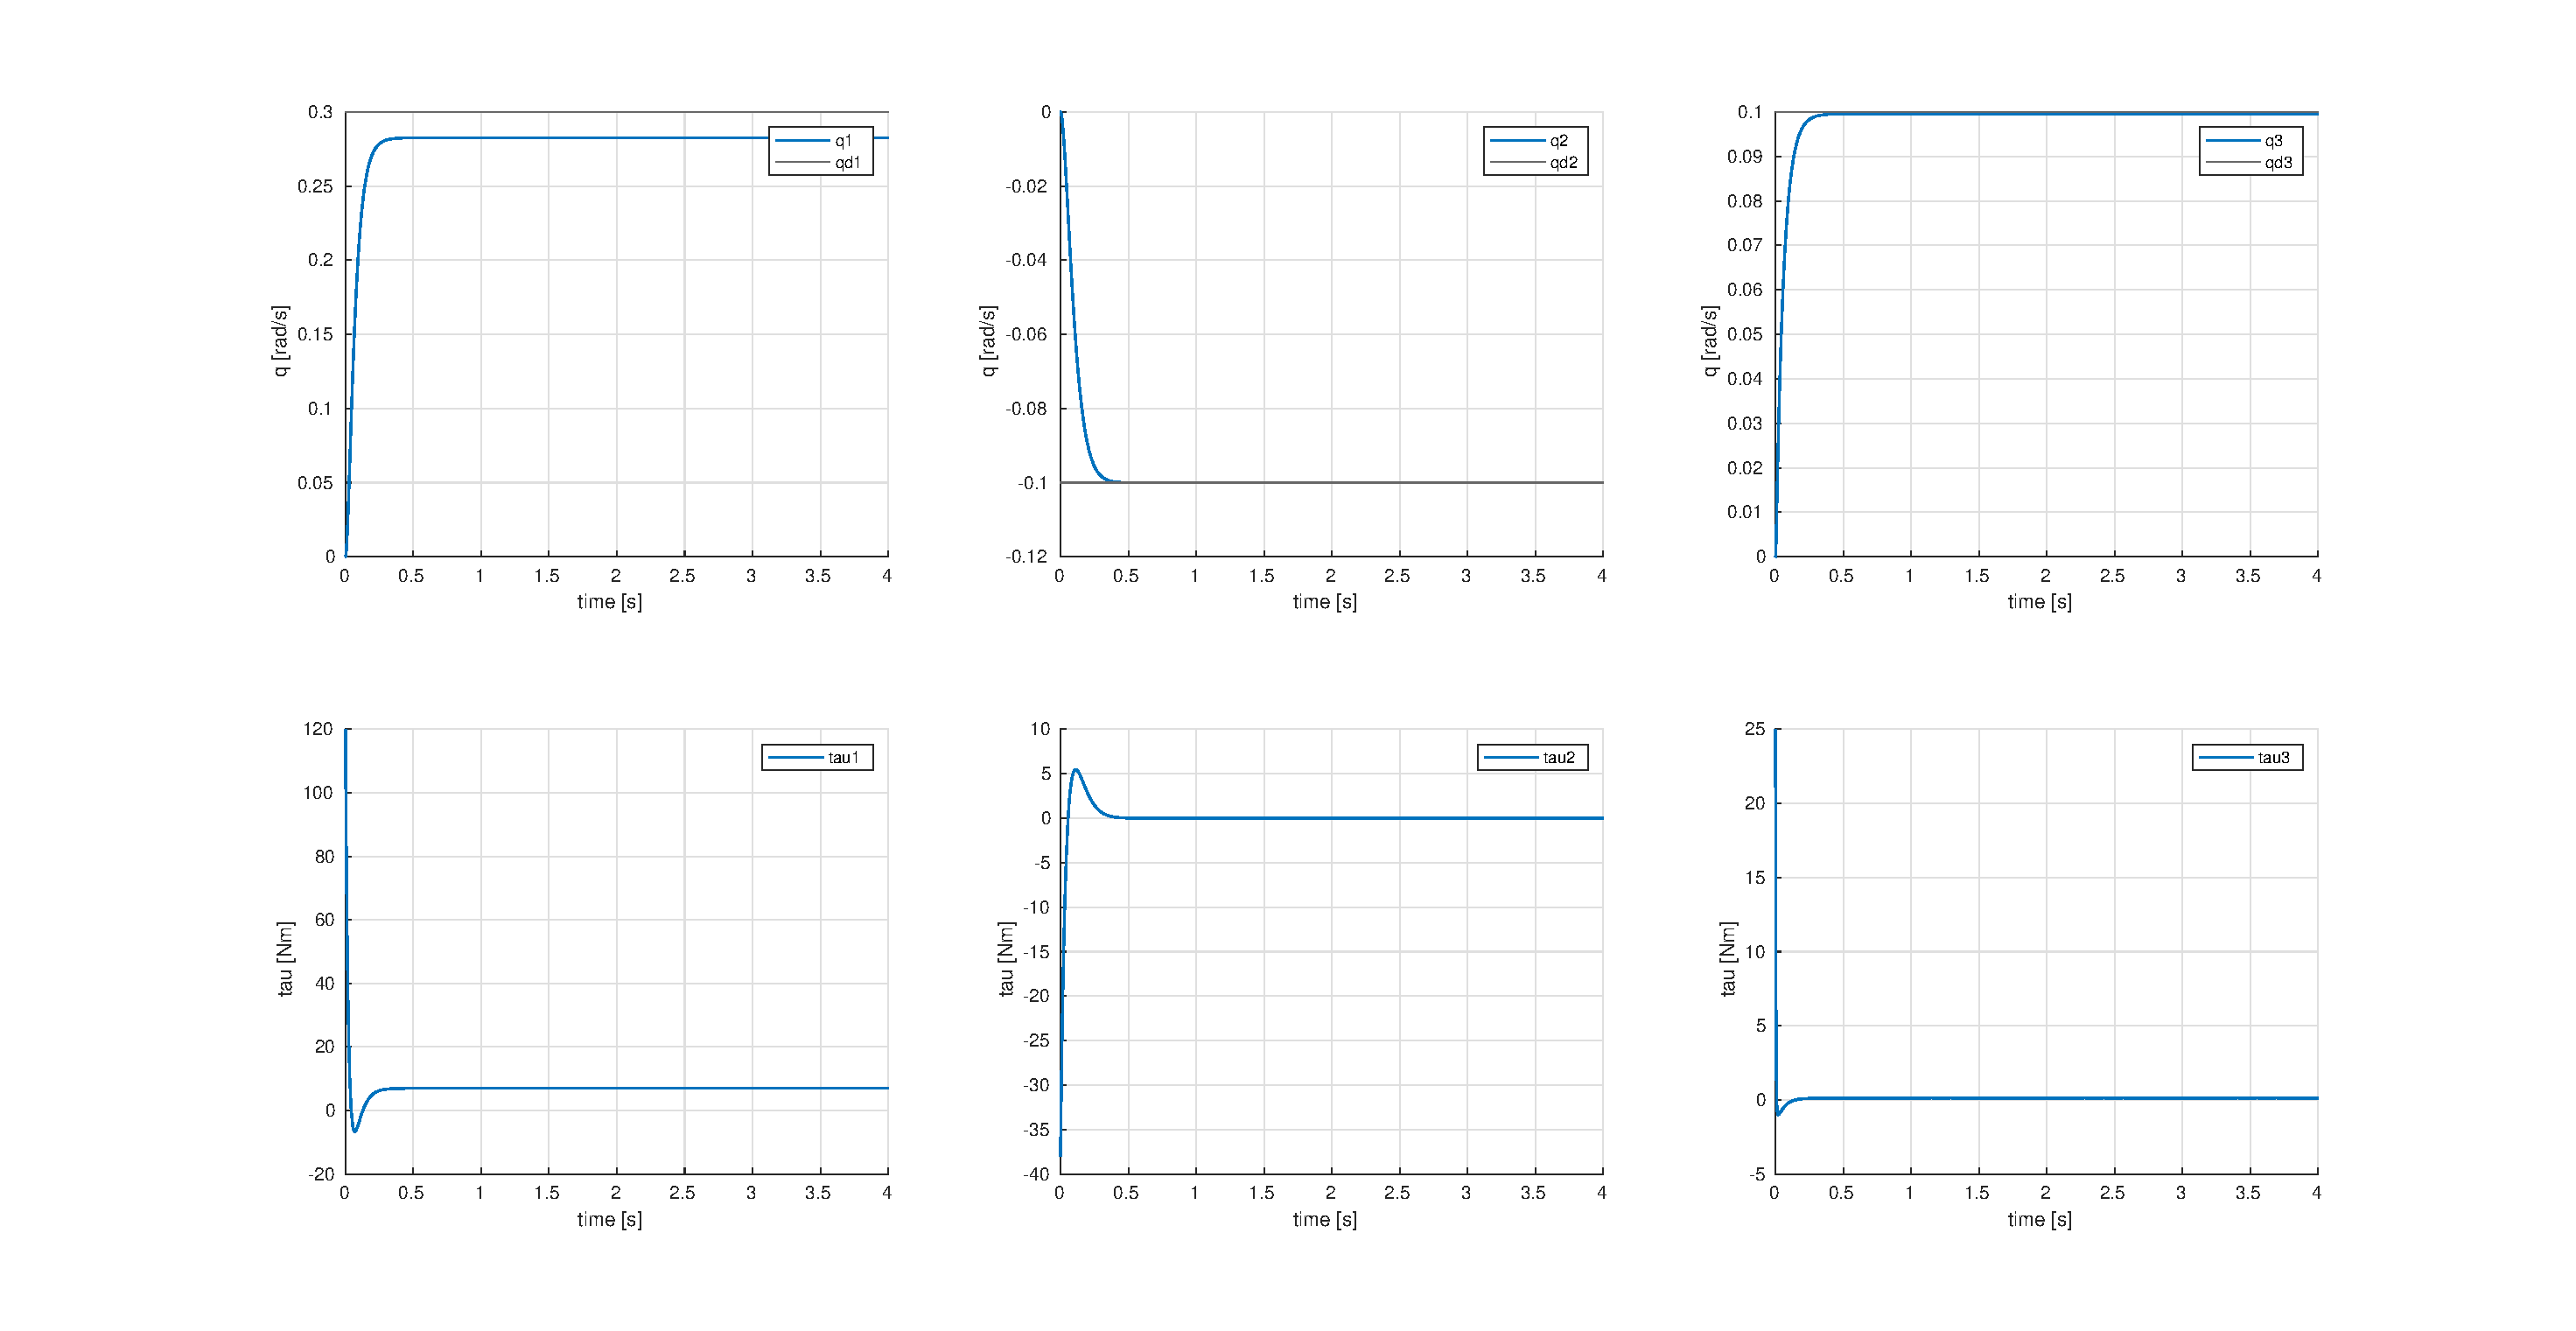
\includegraphics[scale=0.5]{images/gravity_comp_no_gravity.eps}
    \end{center}
    \caption{Joint Space PD Control without Gravity Compensation}
    \label{fig:gravity_comp_no_gravity}
\end{figure}

\newpage
\subsubsection{With fixed $q_d$ for gravity compensation}
Finally let's compare the result obtained with gravity with fixed or time-varying $q_d$. In Fig \ref{fig:gravity_comp_fixed} a small portion of the response of the first joint is reported to show the small differences using a fixed $q_d$ for the gravity compensation vs the time-varying one.

\begin{figure}[H]
    \begin{center}
        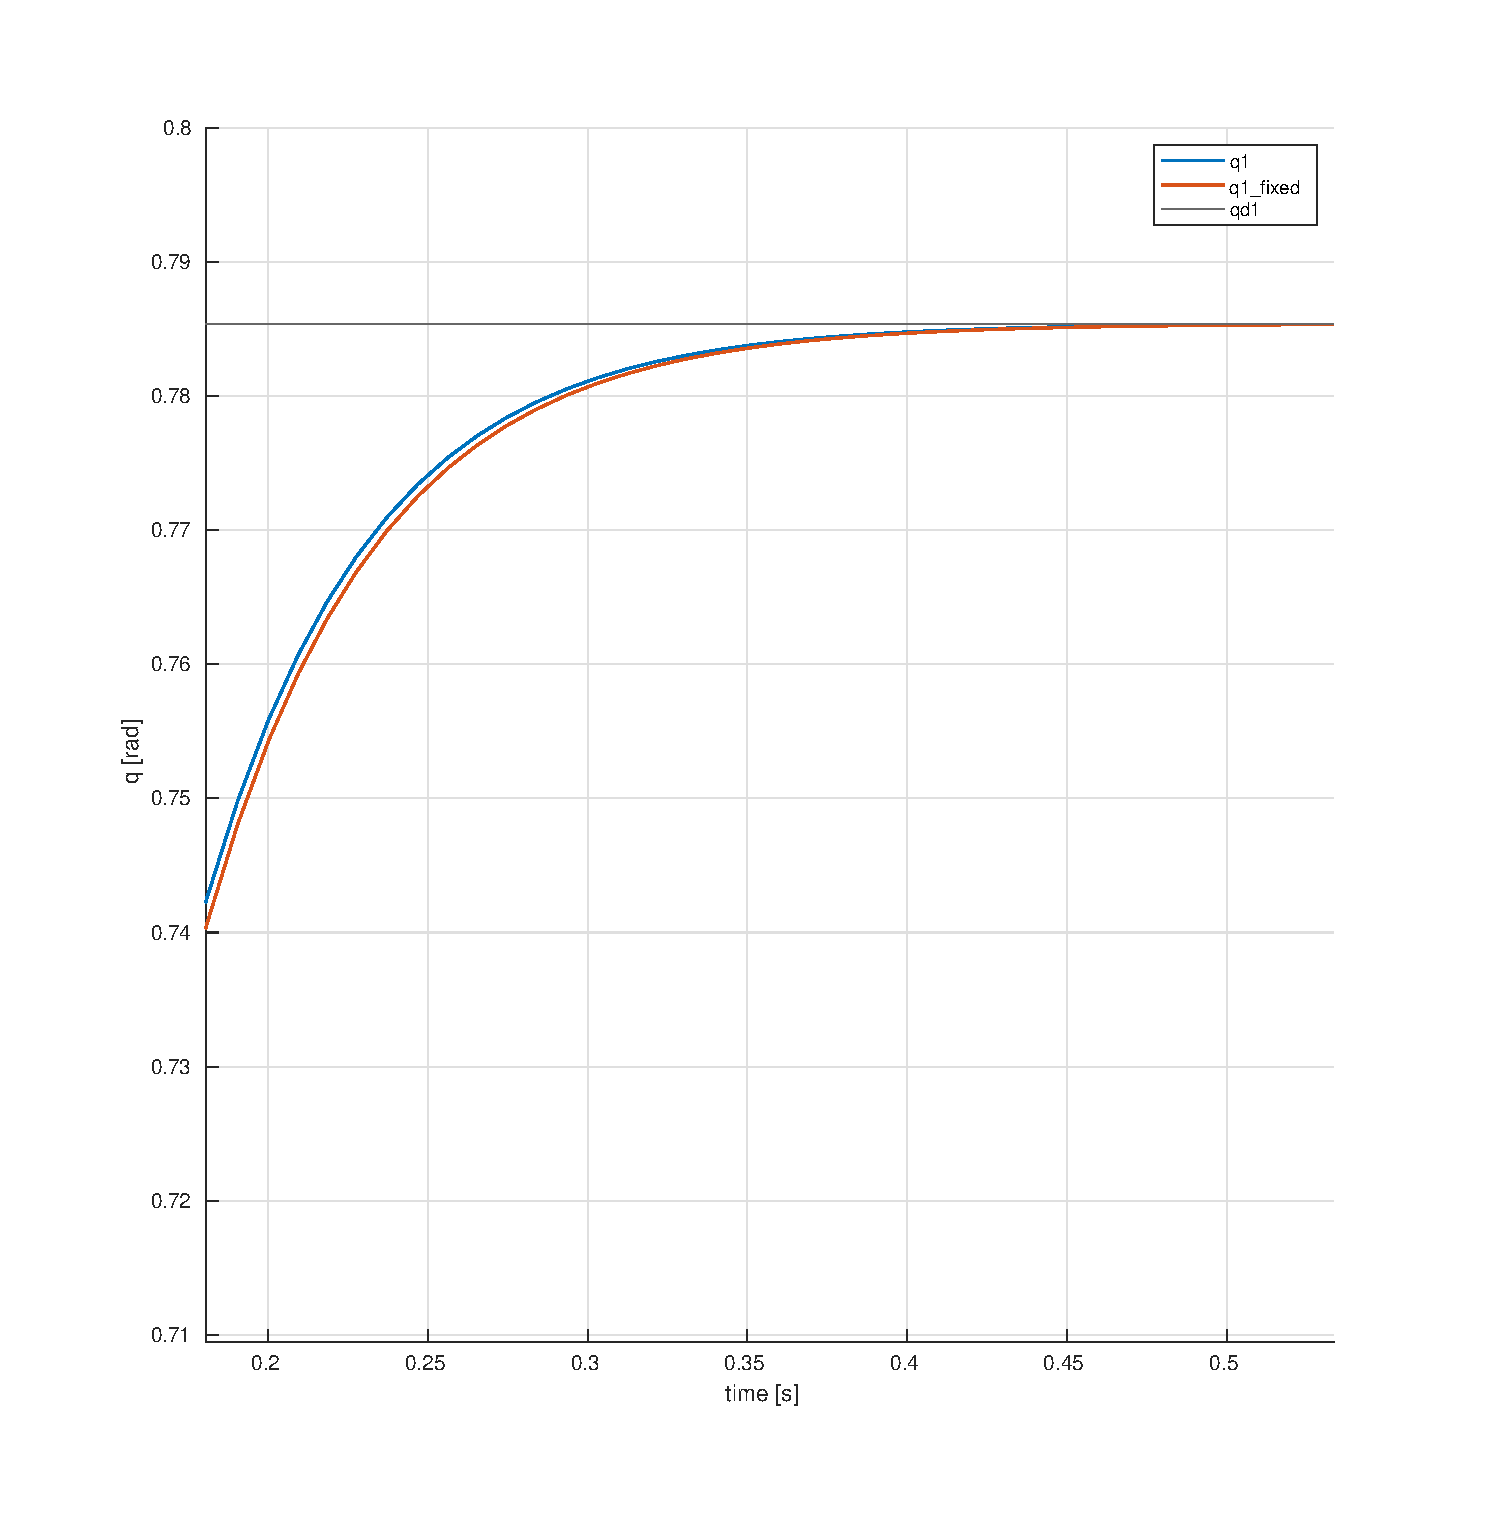
\includegraphics[scale=0.4]{images/gravity_comp_fixed.eps}
    \end{center}
    \caption{Joint Space PD Control with Gravity and fixed vs variable $q_d$}
    \label{fig:gravity_comp_fixed}
\end{figure}

\subsubsection{For the tracking problem}

This control architecture can also be used, with acceptable results, for the tracking error if we don't need perfect results. The step response was achived with zero steady-state error thanks to the internal model principle (an integrator is embedded into the system thanks to the gravity compensation). This is not true, for example, for a sinusoidal function and the response is always late with respect of the reference signal. This behaviour is reported in Fig \ref{fig:gravity_comp_tracking}.

\begin{figure}[H]
    \begin{center}
        \hspace*{-4.5cm}
        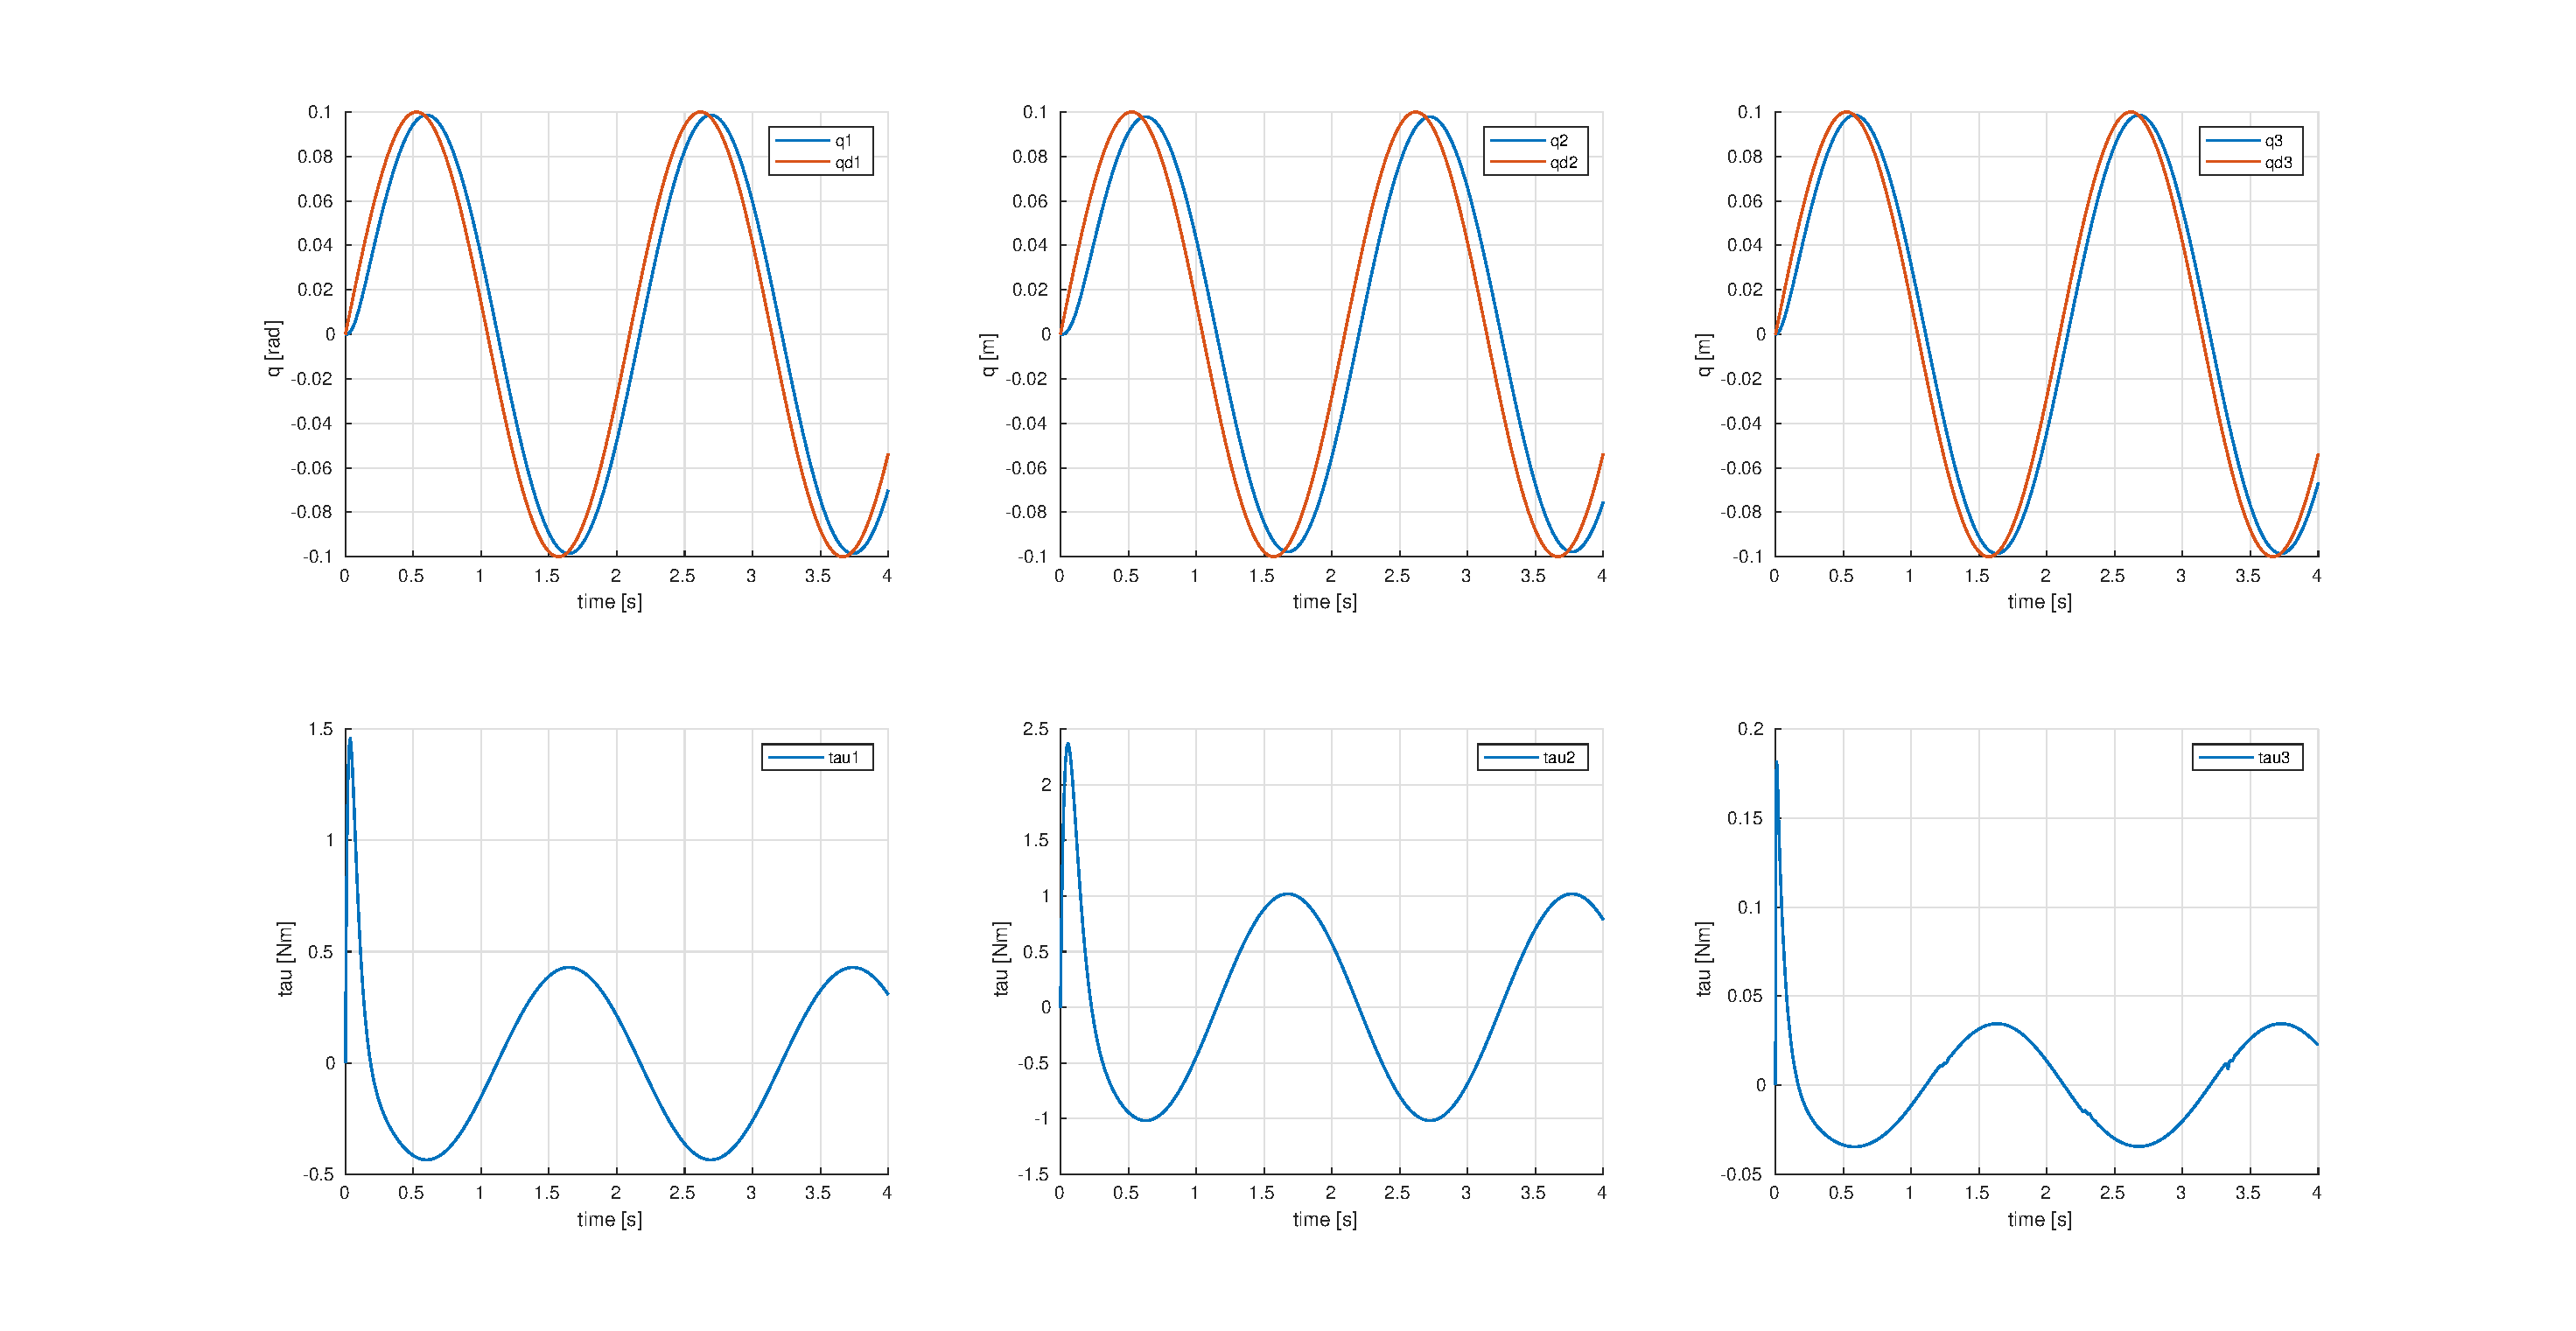
\includegraphics[scale=0.5]{images/gravity_comp_tracking.eps}
    \end{center}
    \caption{Joint Space PD Control with Gravity Compensation for tracking problem}
    \label{fig:gravity_comp_tracking}
\end{figure}

\subsubsection{With gravity compensation and noisy reference}

Finally I can set a disturbance to the input as a sinuoidal function and see the effect on the torque of the related joints. The feedback will try to mitigate this effect and counteract this signal. This effect is reported in Fig \ref{fig:gravity_comp_noise}.

\begin{figure}[H]
    \begin{center}
        \hspace*{-4.5cm}
        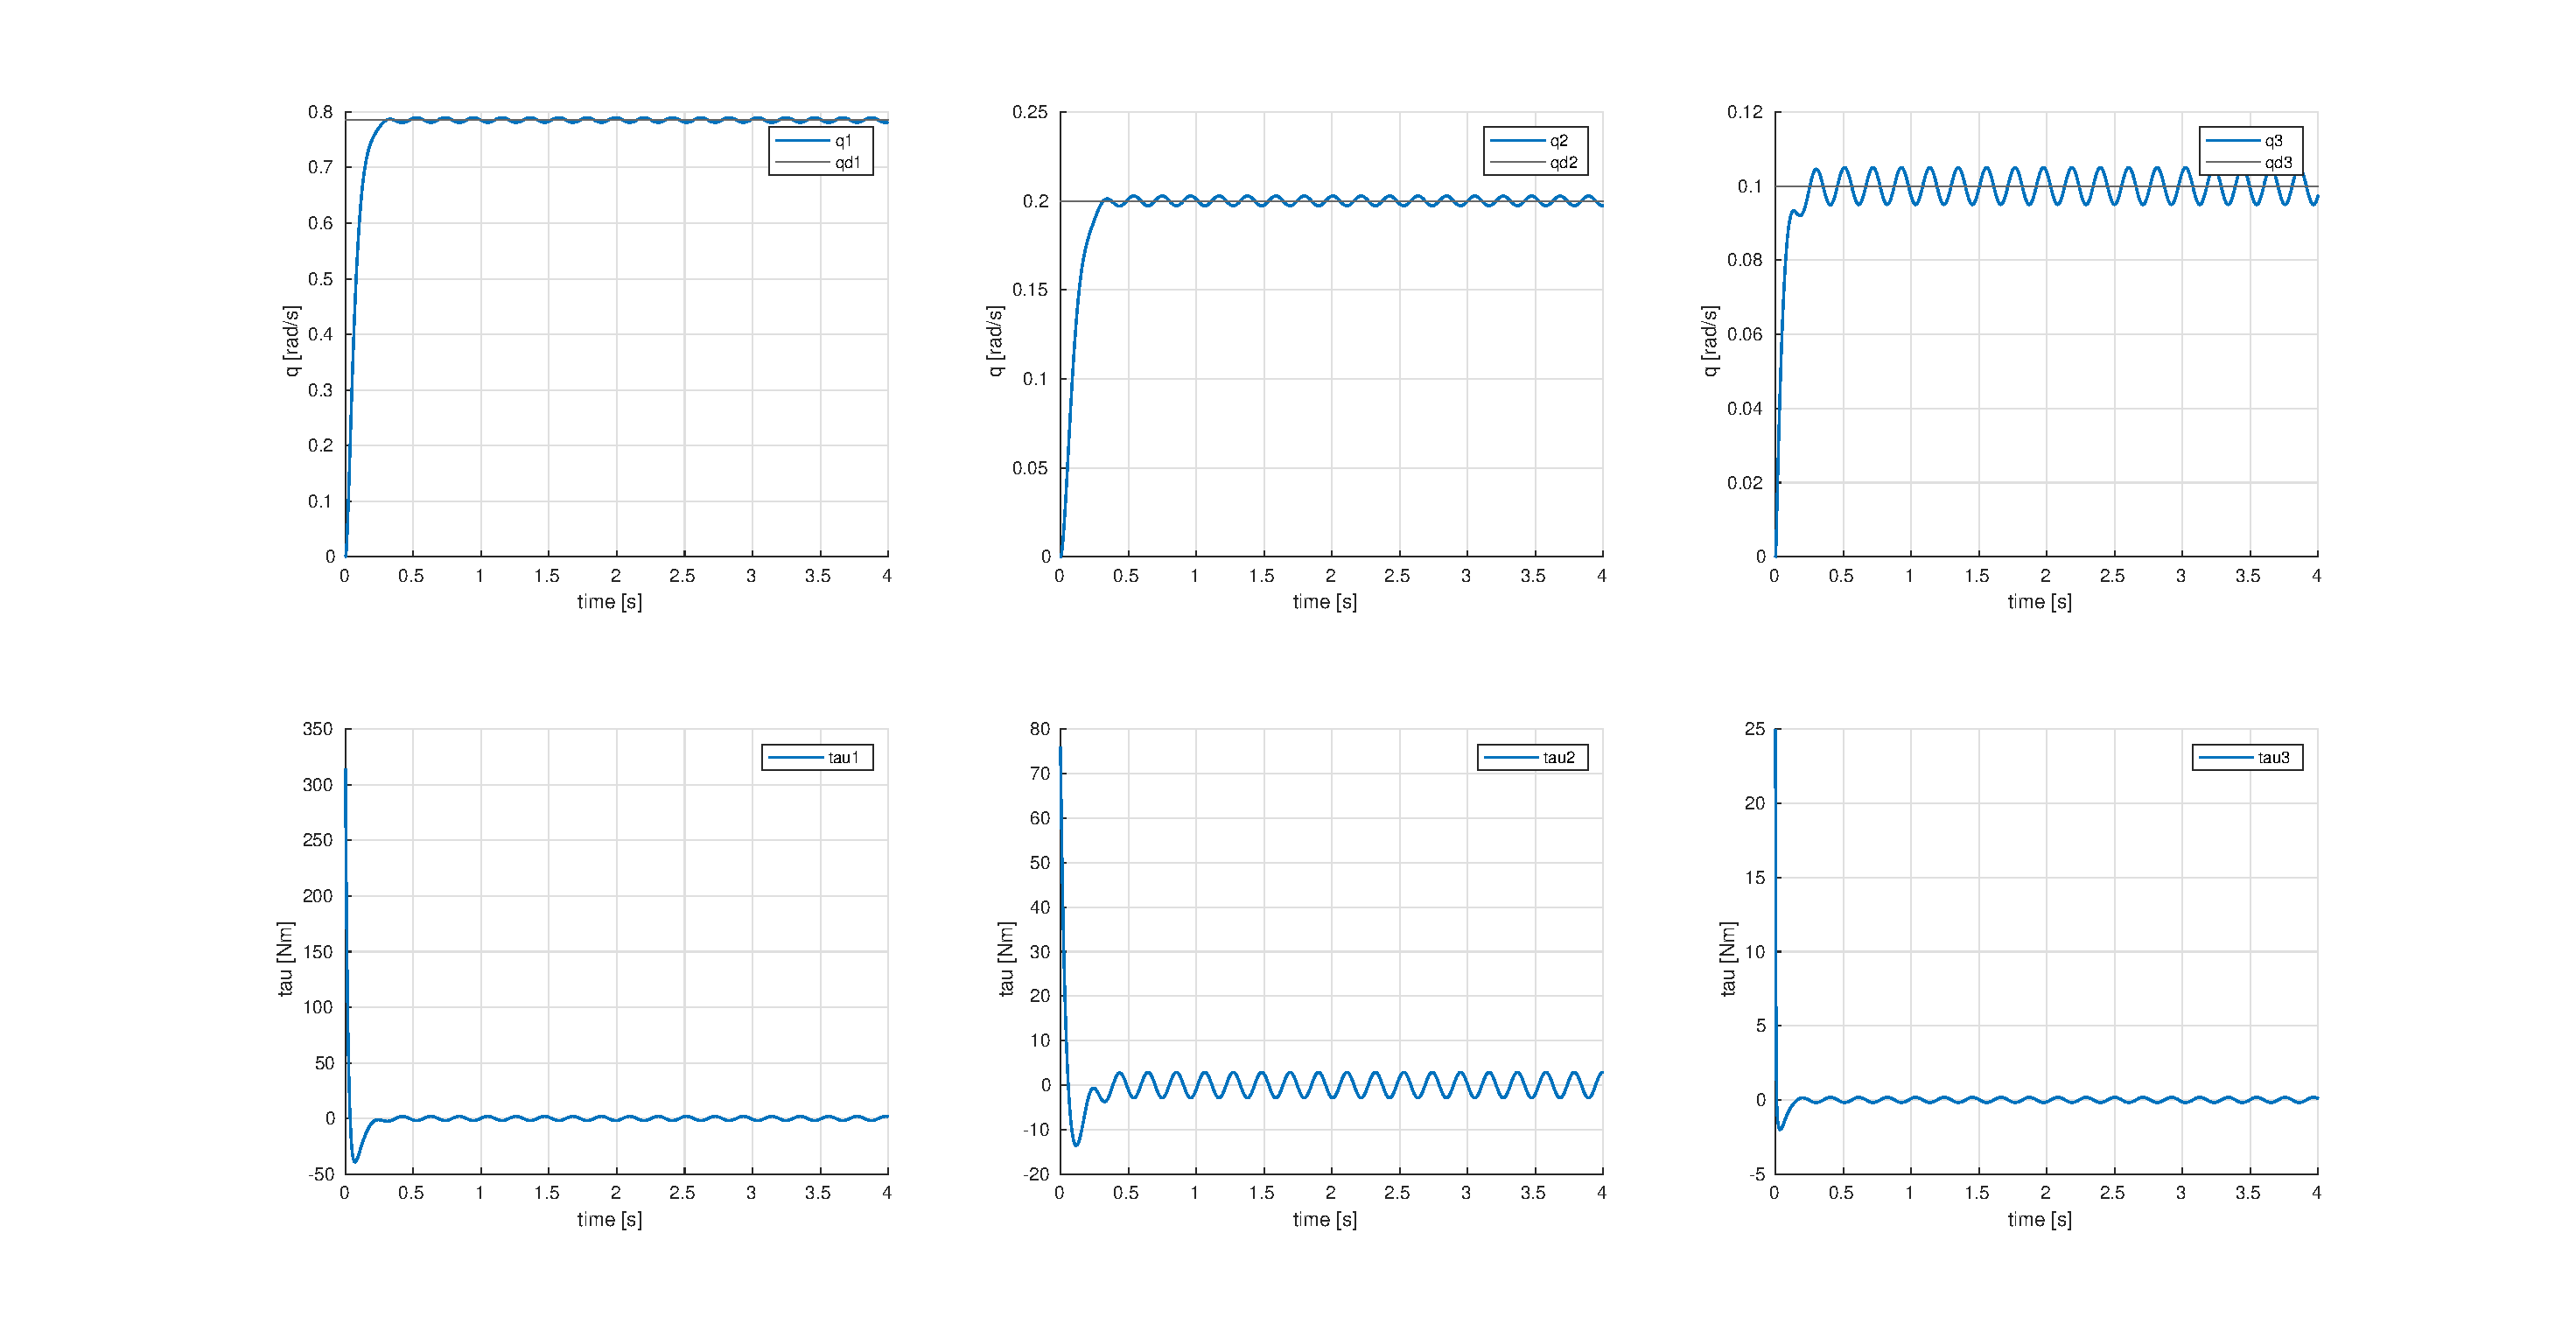
\includegraphics[scale=0.5]{images/gravity_comp_noise.eps}
    \end{center}
    \caption{Joint Space PD Control with Gravity Compensation with noisy reference}
    \label{fig:gravity_comp_noise}
\end{figure}

\begin{theorem}
A PD controller with gravity compensation
\[
    u = g(q_{d}) + K_p(q_d -q) - K_d\dot{q}
\]
guarantees that the equilibrium point $(q_d, 0)$ on the system 
\[
    B(q)\ddot{q} + C(q,\dot{q}) \dot{q} + F\dot{q} + g(q) = u
\]
is globally asymptotically stable
\end{theorem}

It is important to notice that the control law requires the on-line computation of the term $g(q)$, moreover if the matrices $K_p$ and $K_d$ are chosen diagonal we have n decentralized PD controllers, one for each degree of fredom of the robotic manipulator (A PD controlle is a similar to a software spring-damper system)

\newpage 
\subsection{Joint Space Inverse Dynamic PD control}

The joint space inverse dynamics PD control architecture was introduced to solve the tracking problem using the 3DOF manipulator. It consists in a  nonlinear state feedback able to make an exact linearization of the nonlinear system dynamics and a stabilizing linear control. 
\[
    \tau = B(q)y + n(q, \dot{q}) \quad \textbf{inverse dynamics control}
    \qquad
    y = -K_{p}q - K_{d}\dot{q} + r \quad \textbf{stabilizing linear}
\]
where y is the control input of a set of n second order linear and decoupled systems.

In Fig \ref{fig:inv_dyn} and example of the response obtained using a polynomial trajectory with waypoints in (0,3,5) is reported.
\begin{figure}[H]
    \begin{center}
        \hspace*{-4.5cm}
        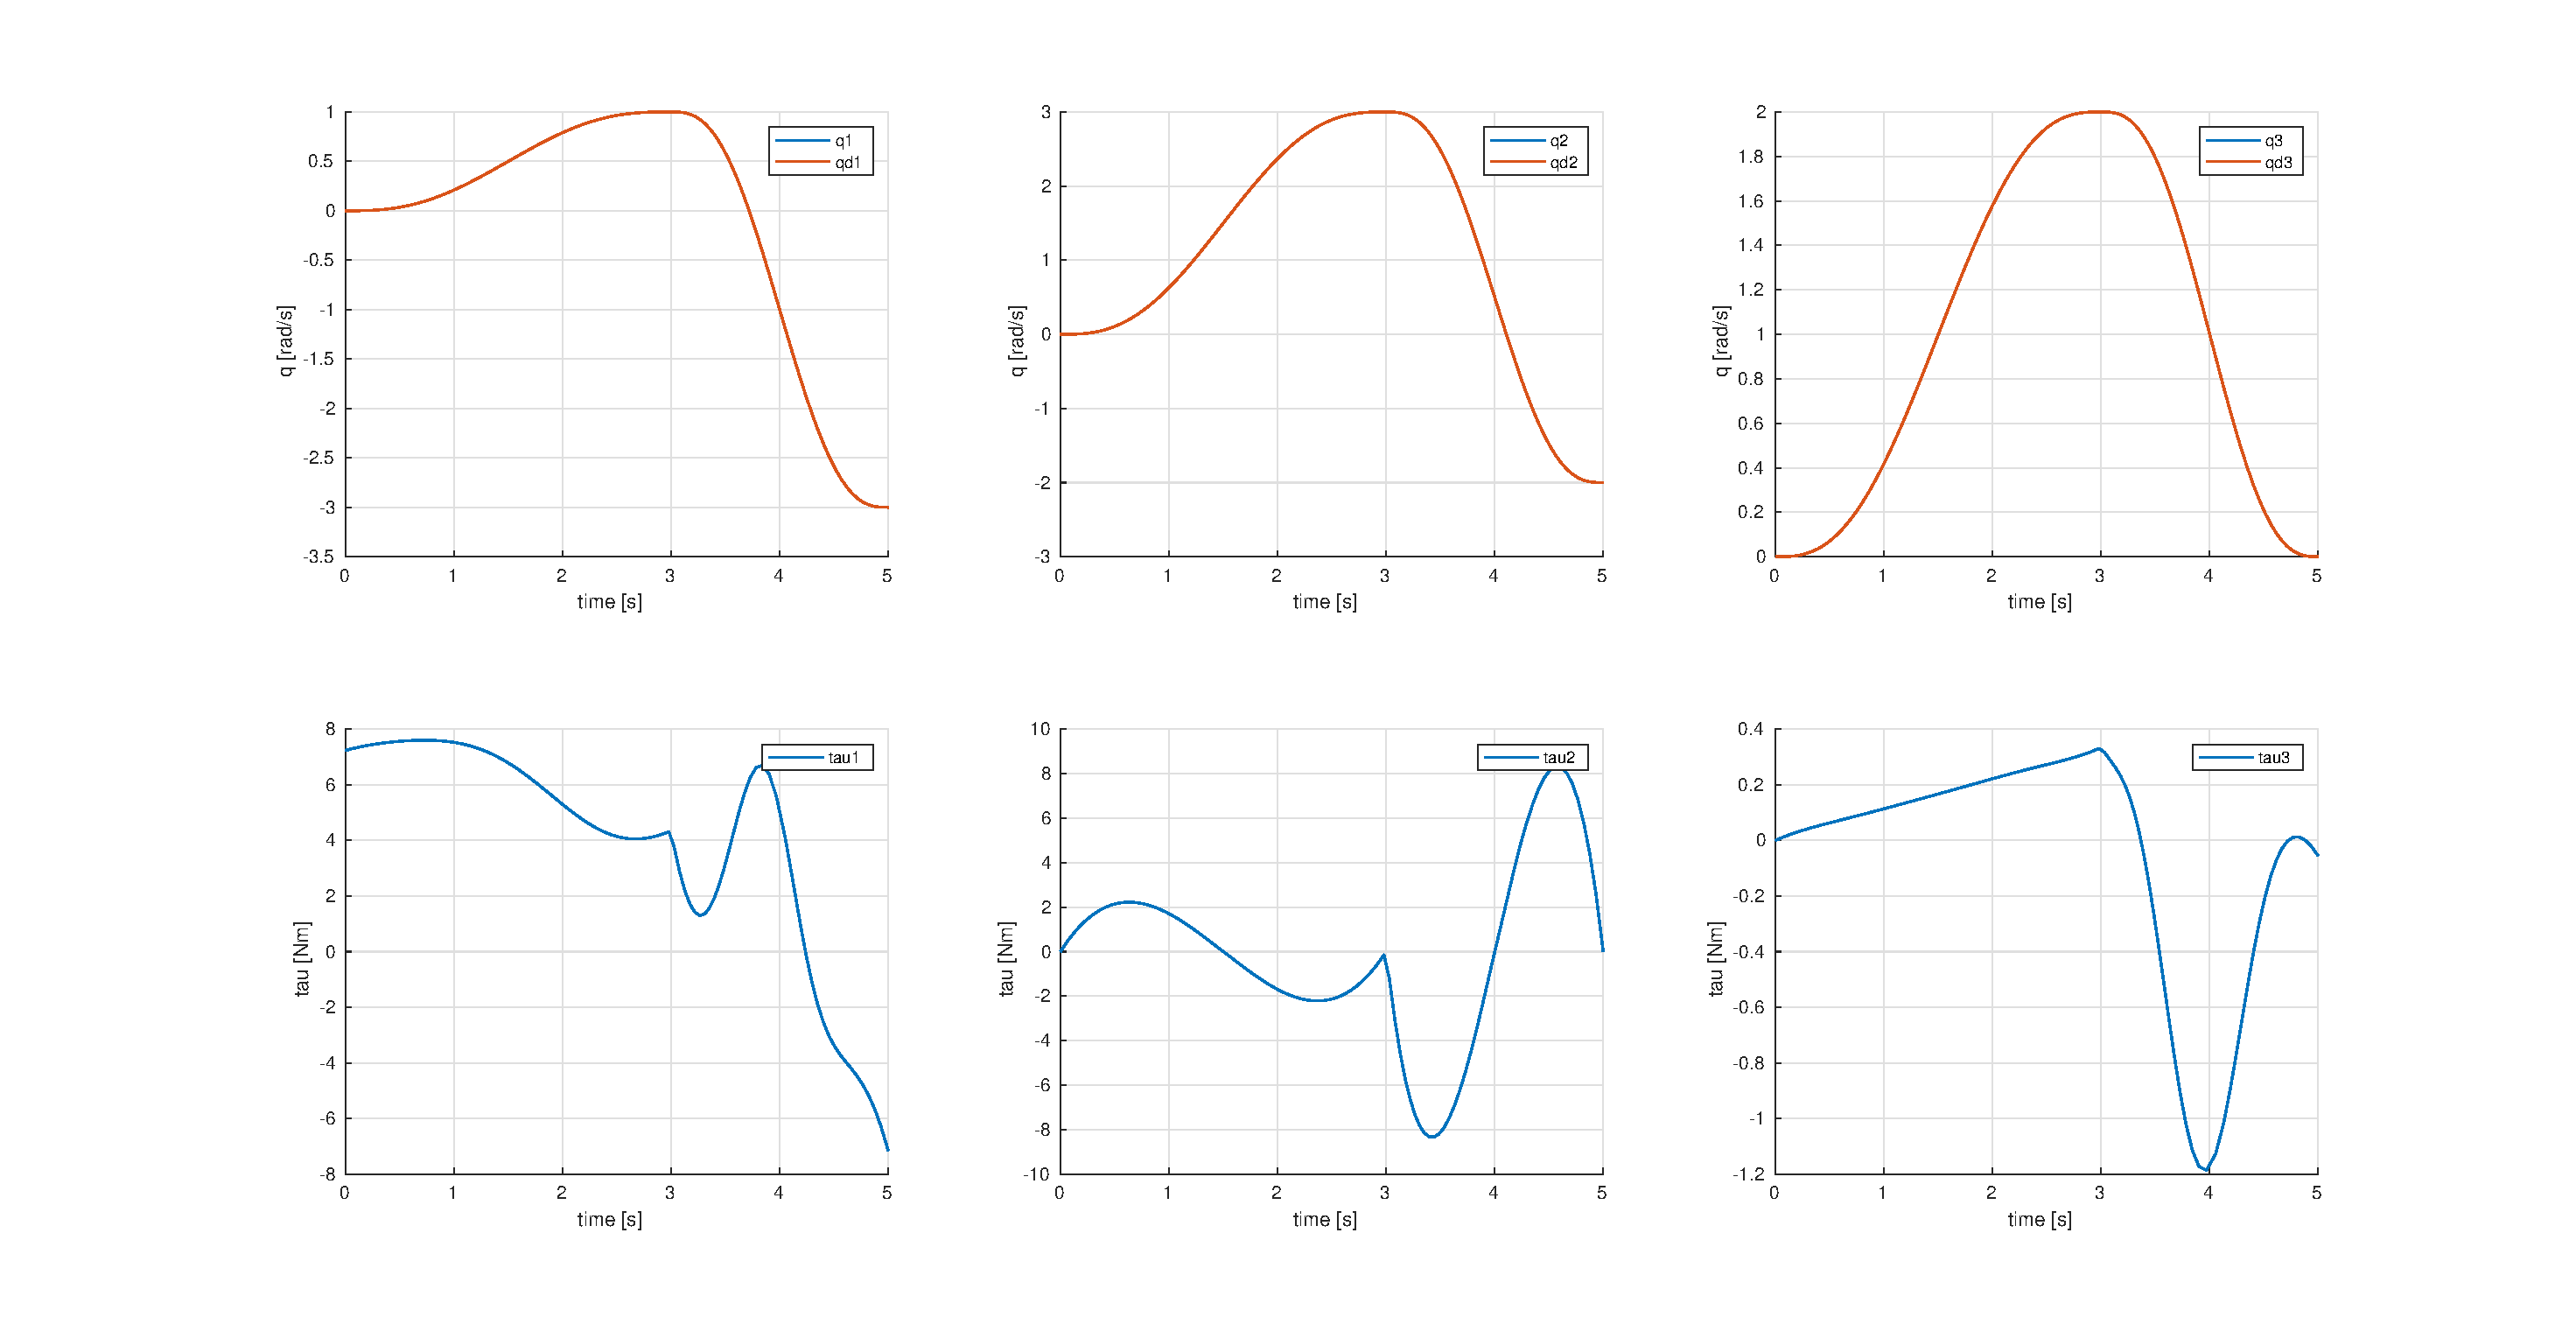
\includegraphics[scale=0.5]{images/inv_dyn.eps}
    \end{center}
    \caption{Inverse dynamic PD control}
    \label{fig:inv_dyn}
\end{figure}

In order to decrease settling time we can increase $K_p$ and $K_d$. Using the perfect linearization (second order system) it looks like we can obtain what we like but it's not true we need too much torque and in real life saturation limits play a big role!

We can try to introduce a saturation in $tau$ with the identical saturation for each joint (in real life it's different for each joint). As a result we obtain huge overshoot and settling time is higher. (Note: we have an integrator in the plant we can't implement an antiwindup in fact we don't have it in the control side).

\subsubsection{With G, B, C different than \^{G}, \^{B}, \^{C}}

\begin{figure}[H]
    \begin{center}
        \hspace*{-4.5cm}
        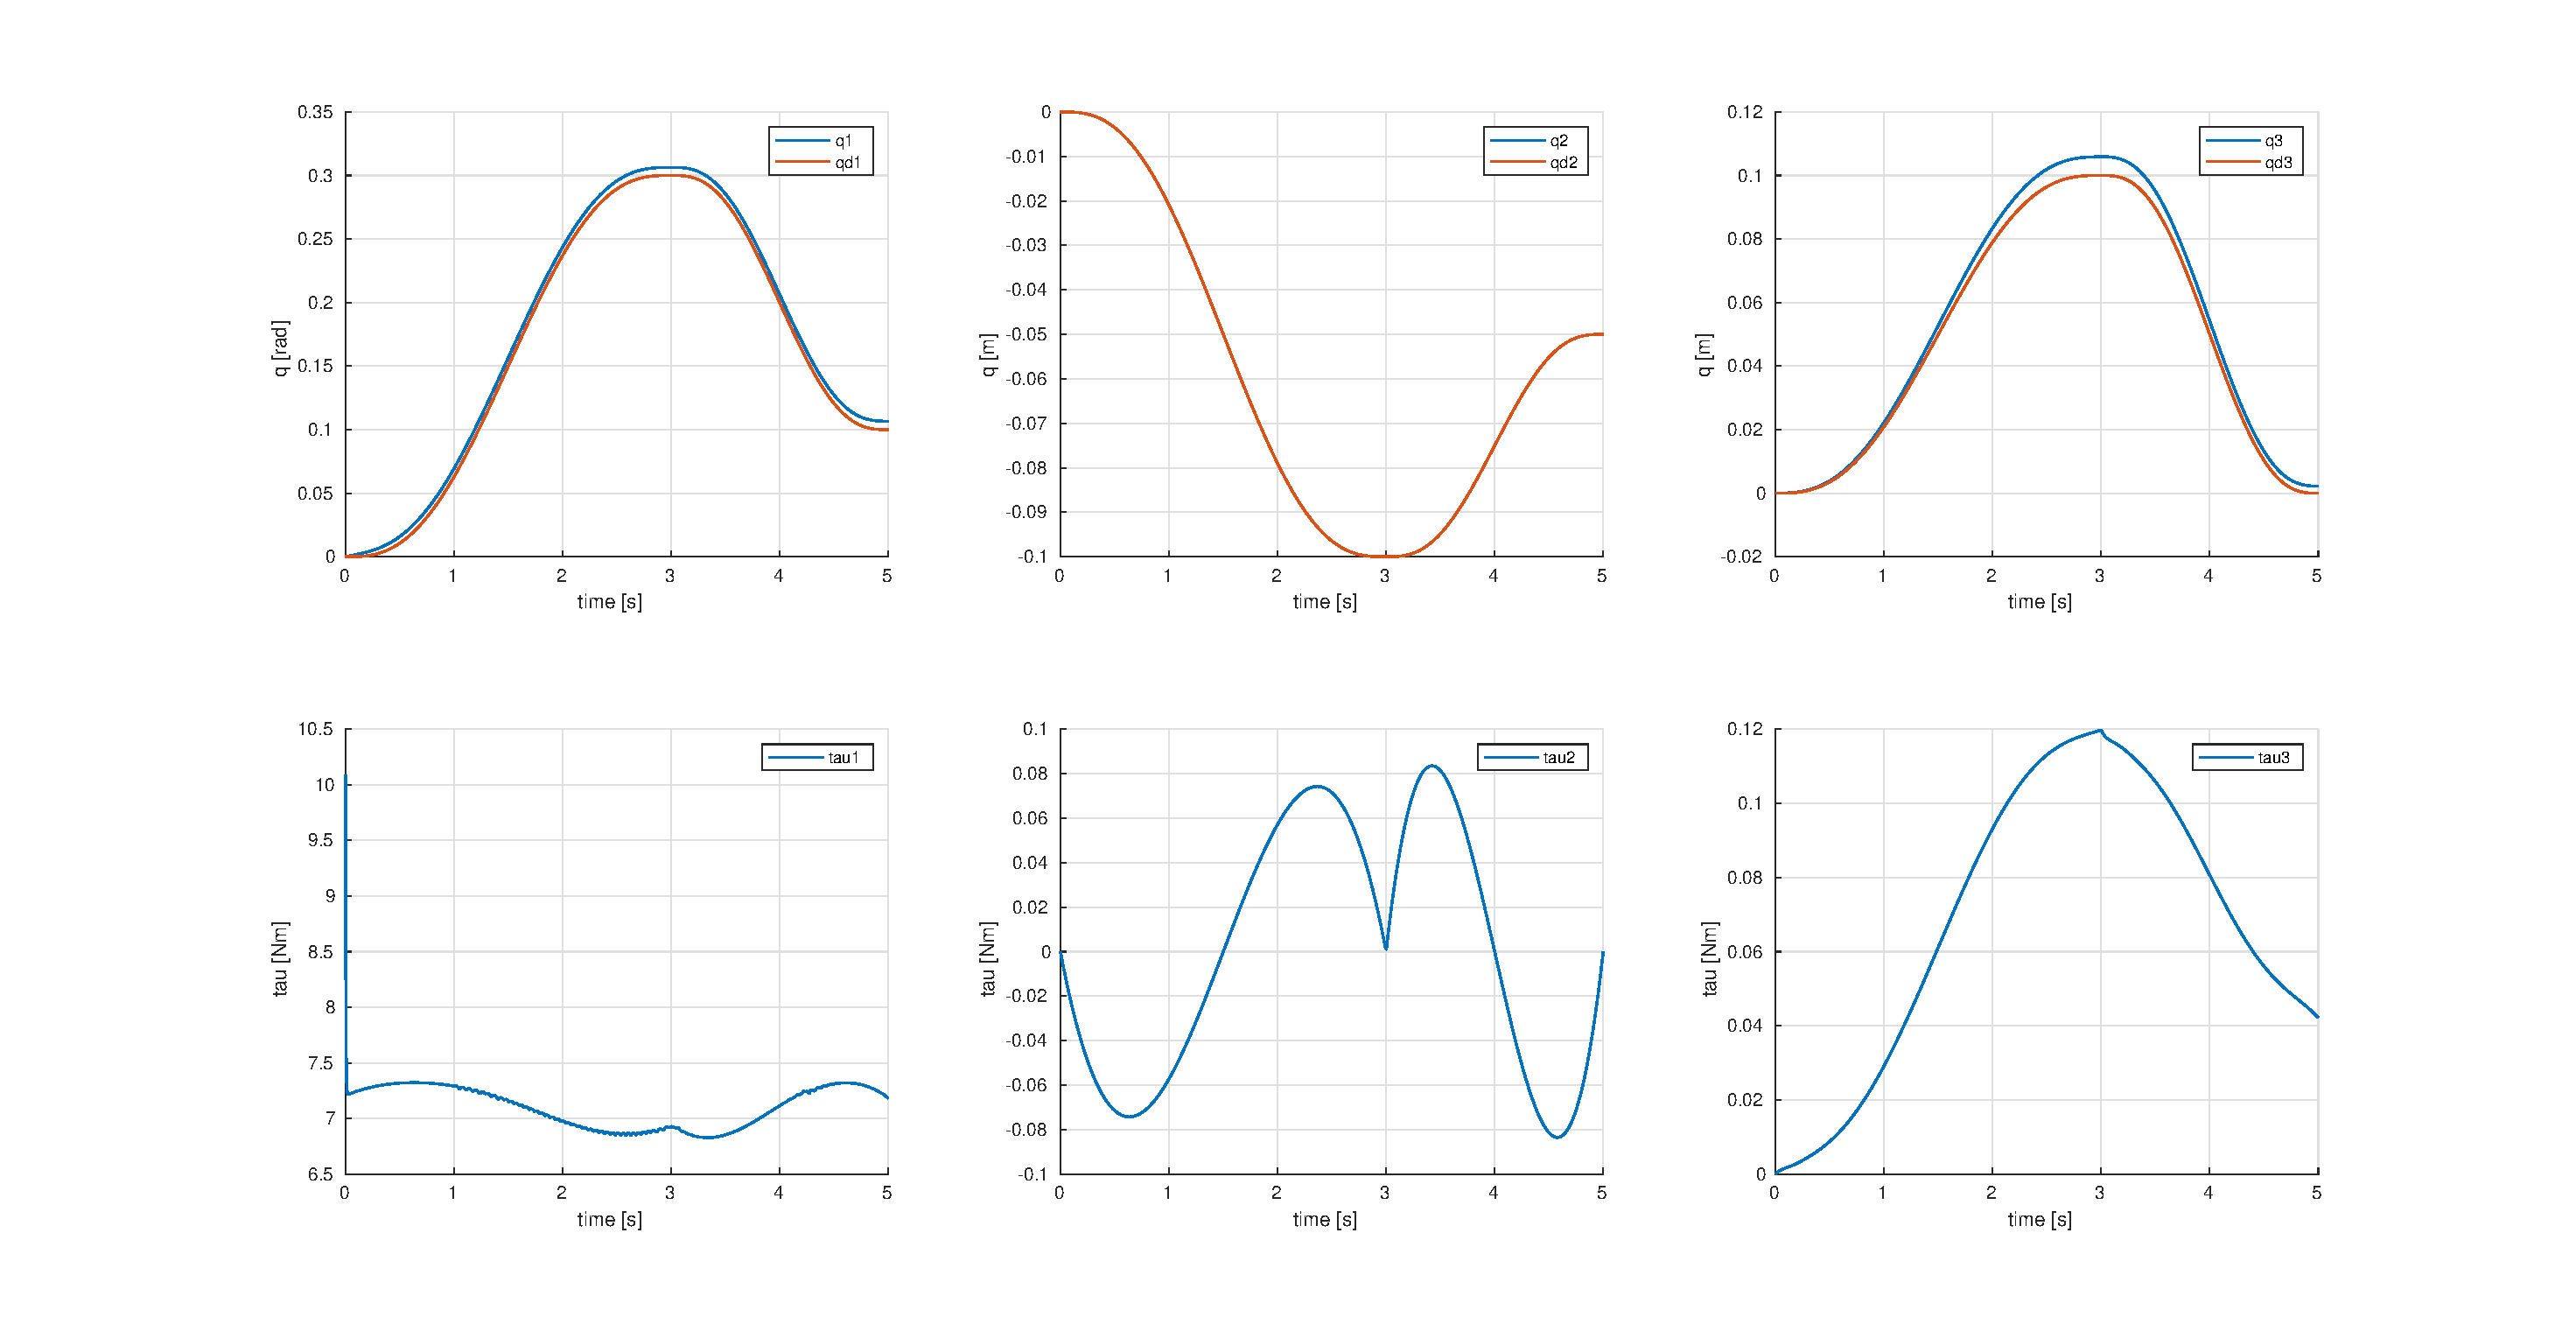
\includegraphics[scale=0.5]{images/inv_dyn_app.eps}
    \end{center}
    \caption{Inverse dynamic PD control with errors in the estimation of the dynamic parameters ($m_1$ and $m_3$ double than the real values)}
    \label{fig:inv_dyn_app}
\end{figure}

From Fig \ref{fig:inv_dyn_app} it is possible to see that the third joint is clearly affected by the wrong estimation. 

\subsubsection{Without gravity term in $n(q,\dot{q})$}

In Fig \ref{fig:inv_dyn_no_grav} the gravity was removed from the $n(q,\dot{q})$ term which strongly affects the joints 1 and 3, joint 2 is not affected by gravity as it is clearly visible.

\begin{figure}[H]
    \begin{center}
        \hspace*{-4.5cm}
        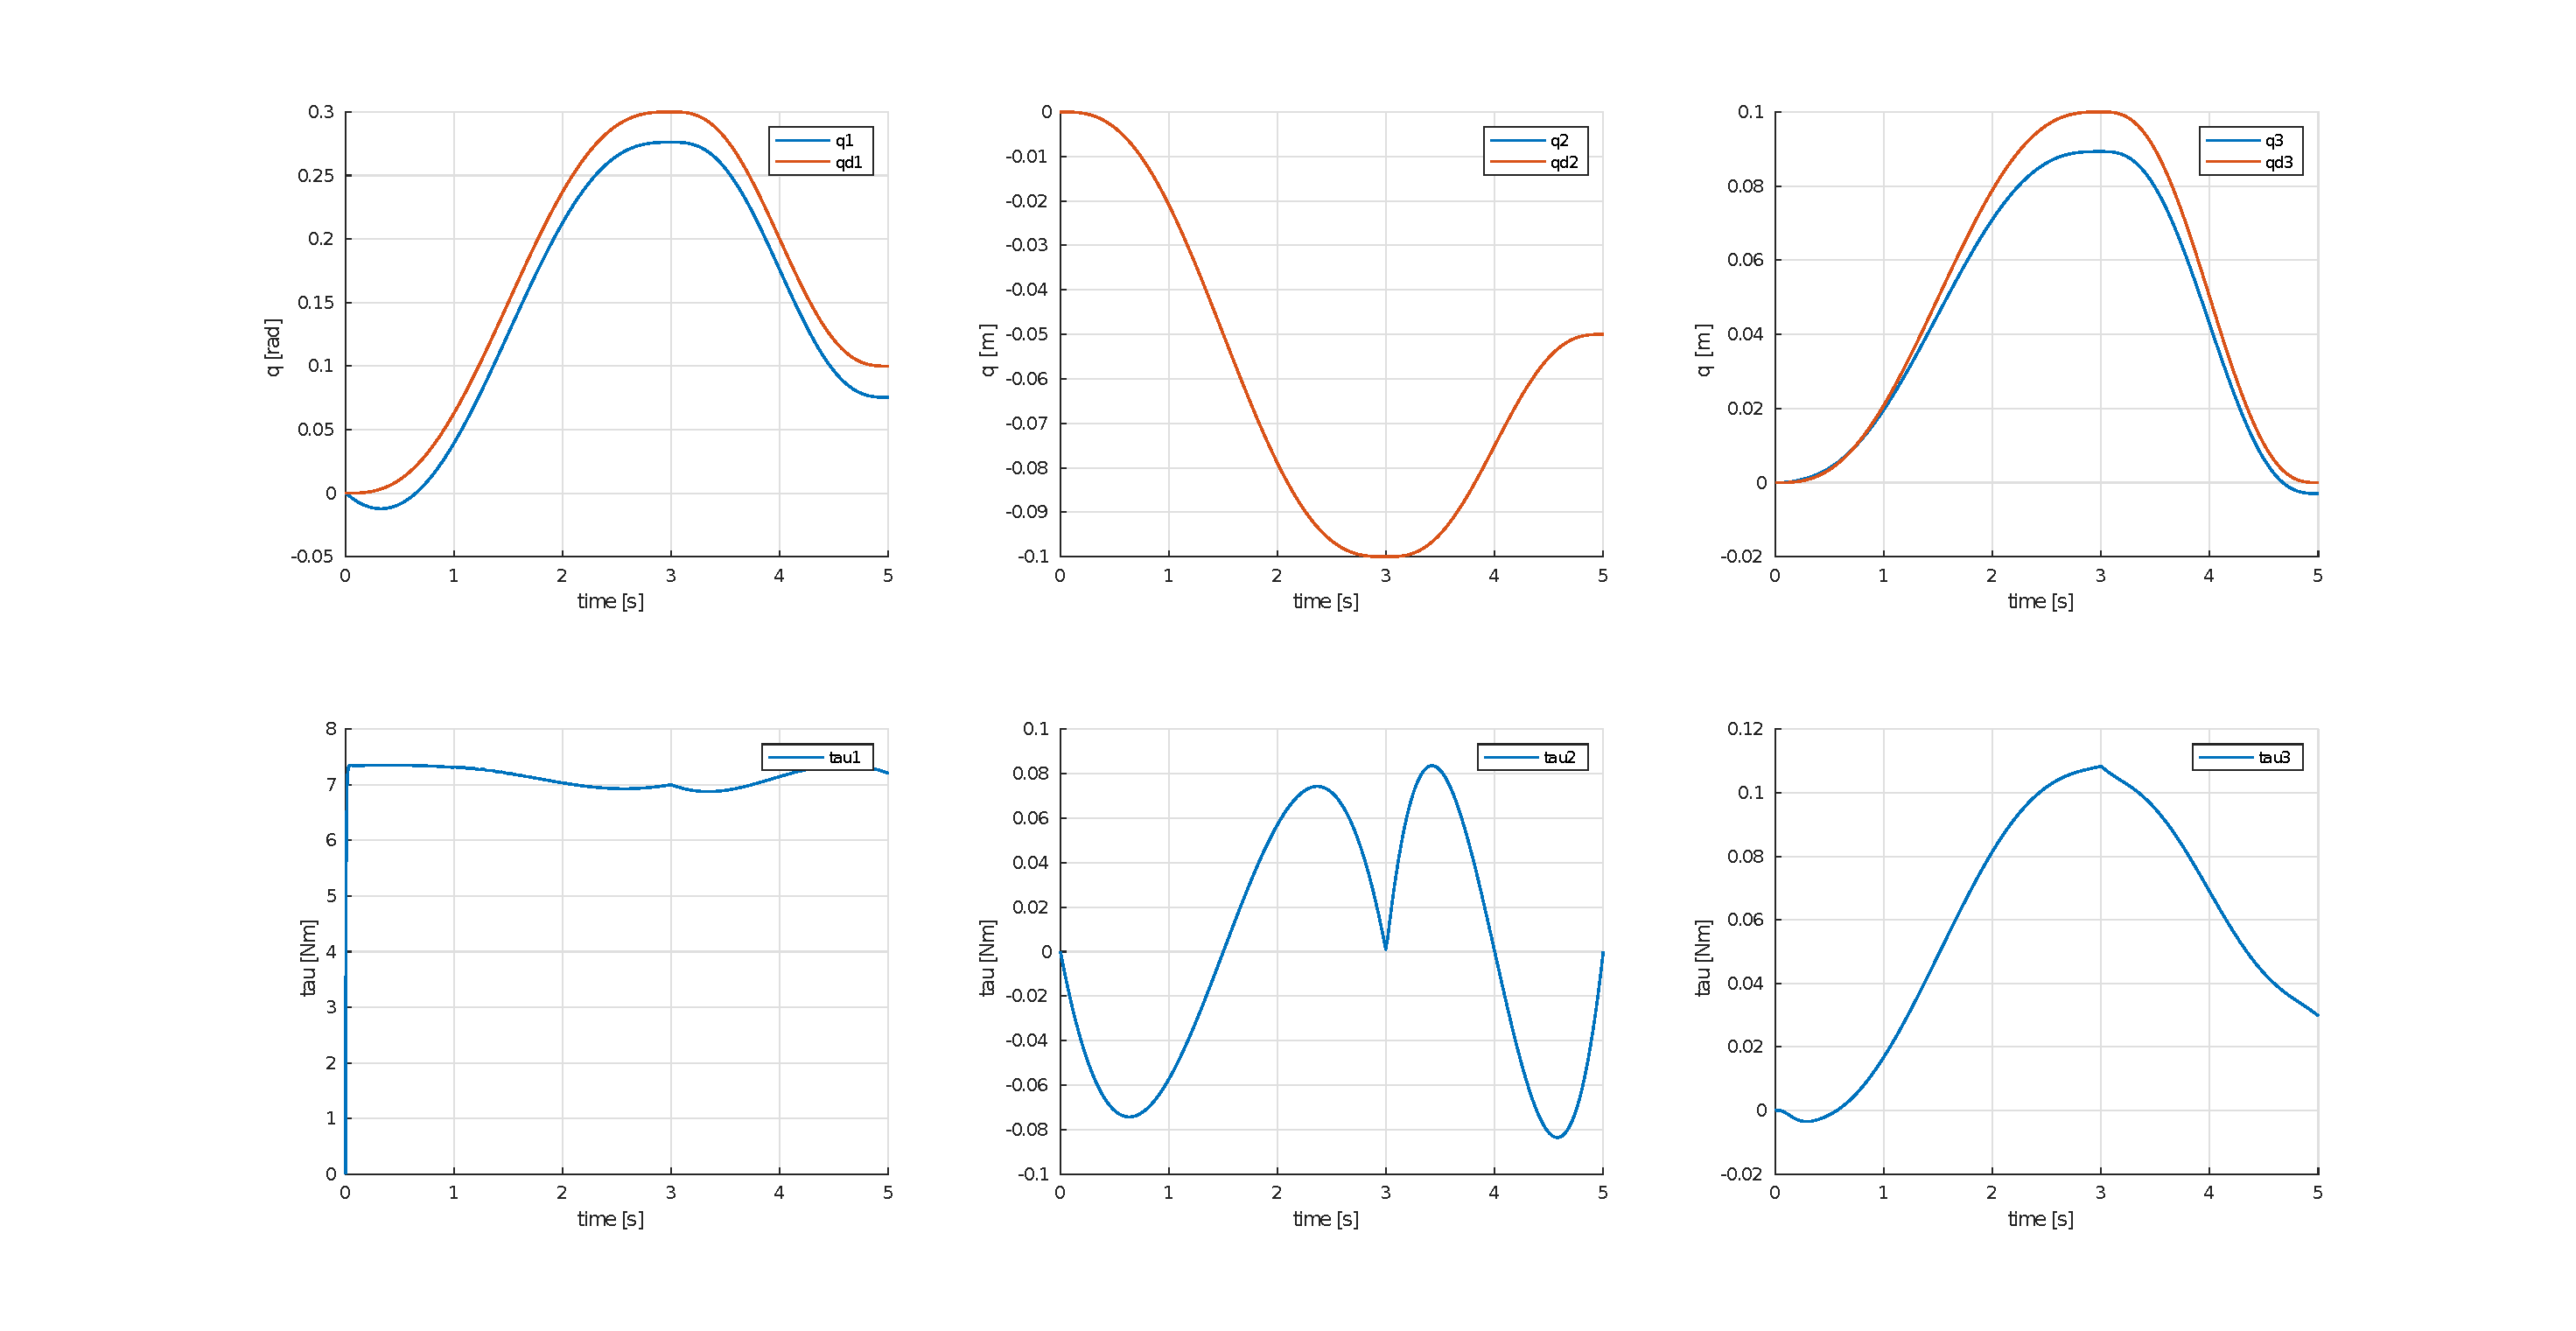
\includegraphics[scale=0.5]{images/inv_dyn_no_grav.eps}
    \end{center}
    \caption{Inverse dynamic PD control without gravity in $n$ term}
    \label{fig:inv_dyn_no_grav}
\end{figure}

\subsubsection{Extra considerations}

\begin{itemize}
\item We can also try to cut $C(q,\dot{q})$ from the architecture and the result in steady state is exactly the same in fact $\dot{q} = 0 $ it doesn't play any role. 

\item We can also try to cut $B(q)$, in this case it is responsible for the decoupling of the joints so if we apply a step to only one joint we should see that without the $B(q)$ the joints are coupled.

\item n time-invariant, linear and decoupled second-order systems. we can choose \[ Kp =  \left \{ w_{n1}^2 , \dots \right \} \] \[ Kd = \left \{2\xi_1 w_{n1}, \dots \right \} \]
\end{itemize}

\newpage
\subsection{Operational Space PD control with gravity compensation}

The result obtained by the PD with gravity compensation in the operational space is reported in Fig \ref{fig:gravity_op}. The robot has 3DOF so it is not possible to force the 3 positions and 3 orientations as we want. To obtained the following results I started from a joint configuration which was translated into the operational space $q = (0.2, 0.2, 0.1)$. The results are provided wrt of frame 0.
\begin{figure}[H]
    \begin{center}
        \hspace*{-4.5cm}
        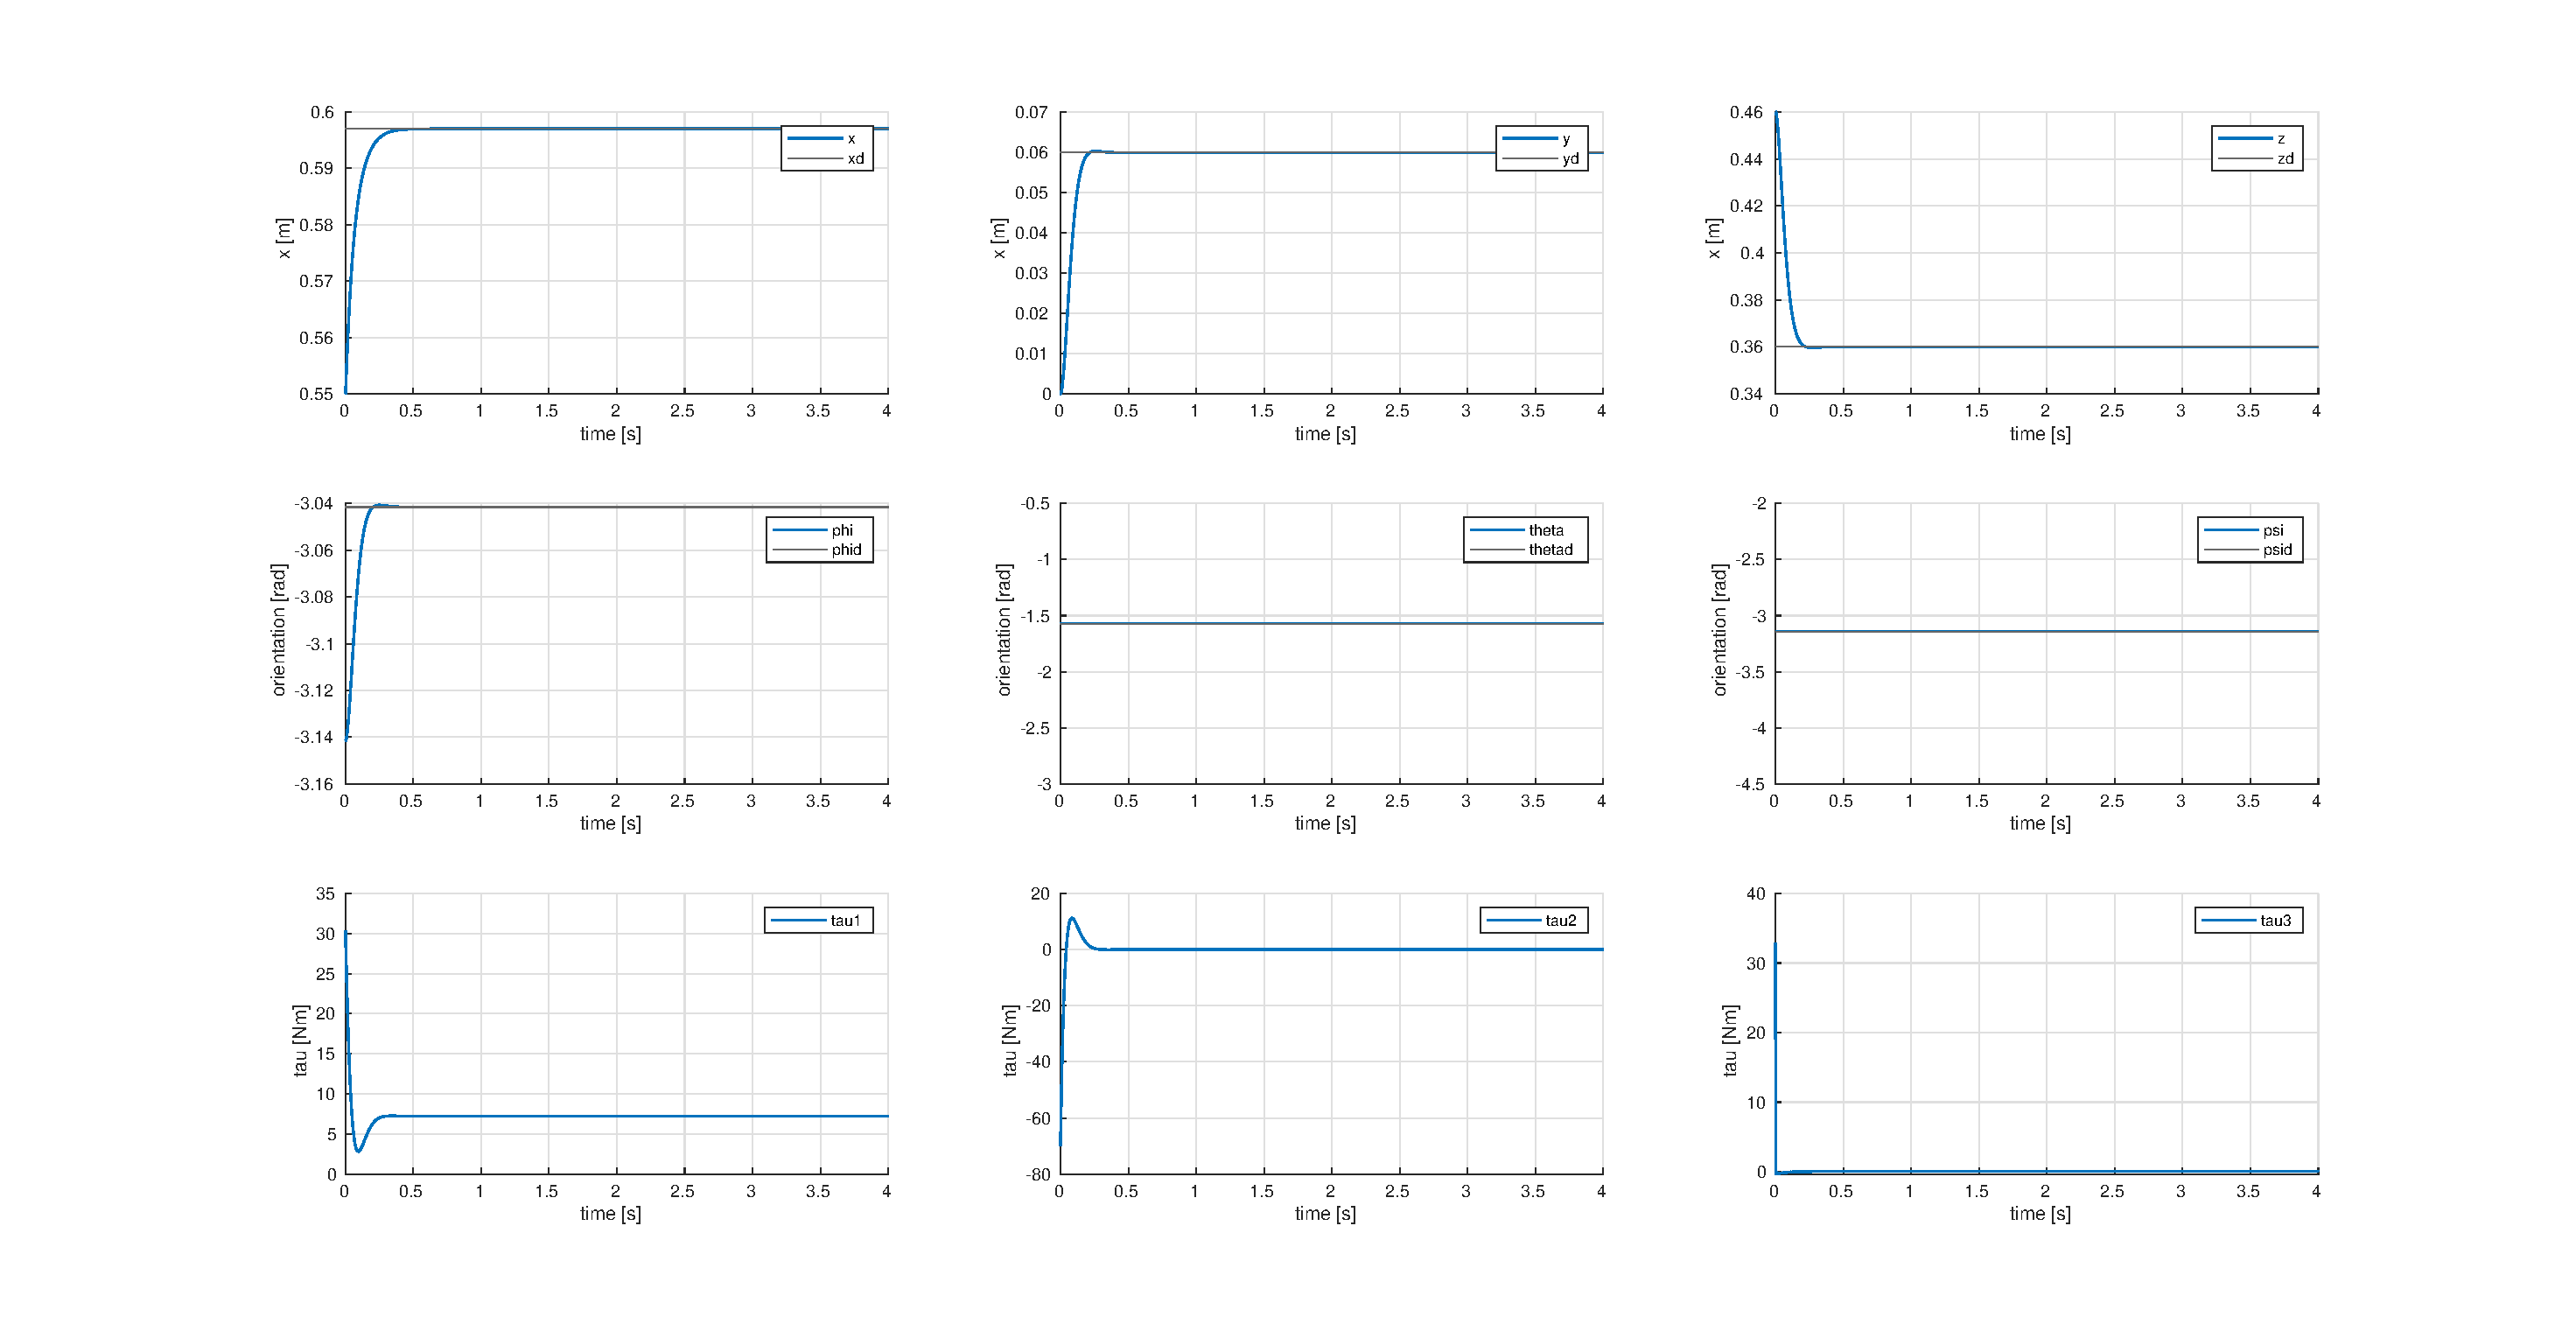
\includegraphics[scale=0.5]{images/op_gravity.eps}
    \end{center}
    \caption{Operational Space PD control with graviy compensation}
    \label{fig:gravity_op}
\end{figure}

\subsubsection{Without gravity}

The desired configuration is $q = (0, 0.2, 0)$ in which the joint 1 and partially joint 3 are responsible for the gravity compensation as it is visible. As it is visible $x$ and $y$ don't compensate anymore (wrt of frame 0).

\begin{figure}[H]
    \begin{center}
        \hspace*{-4.5cm}
        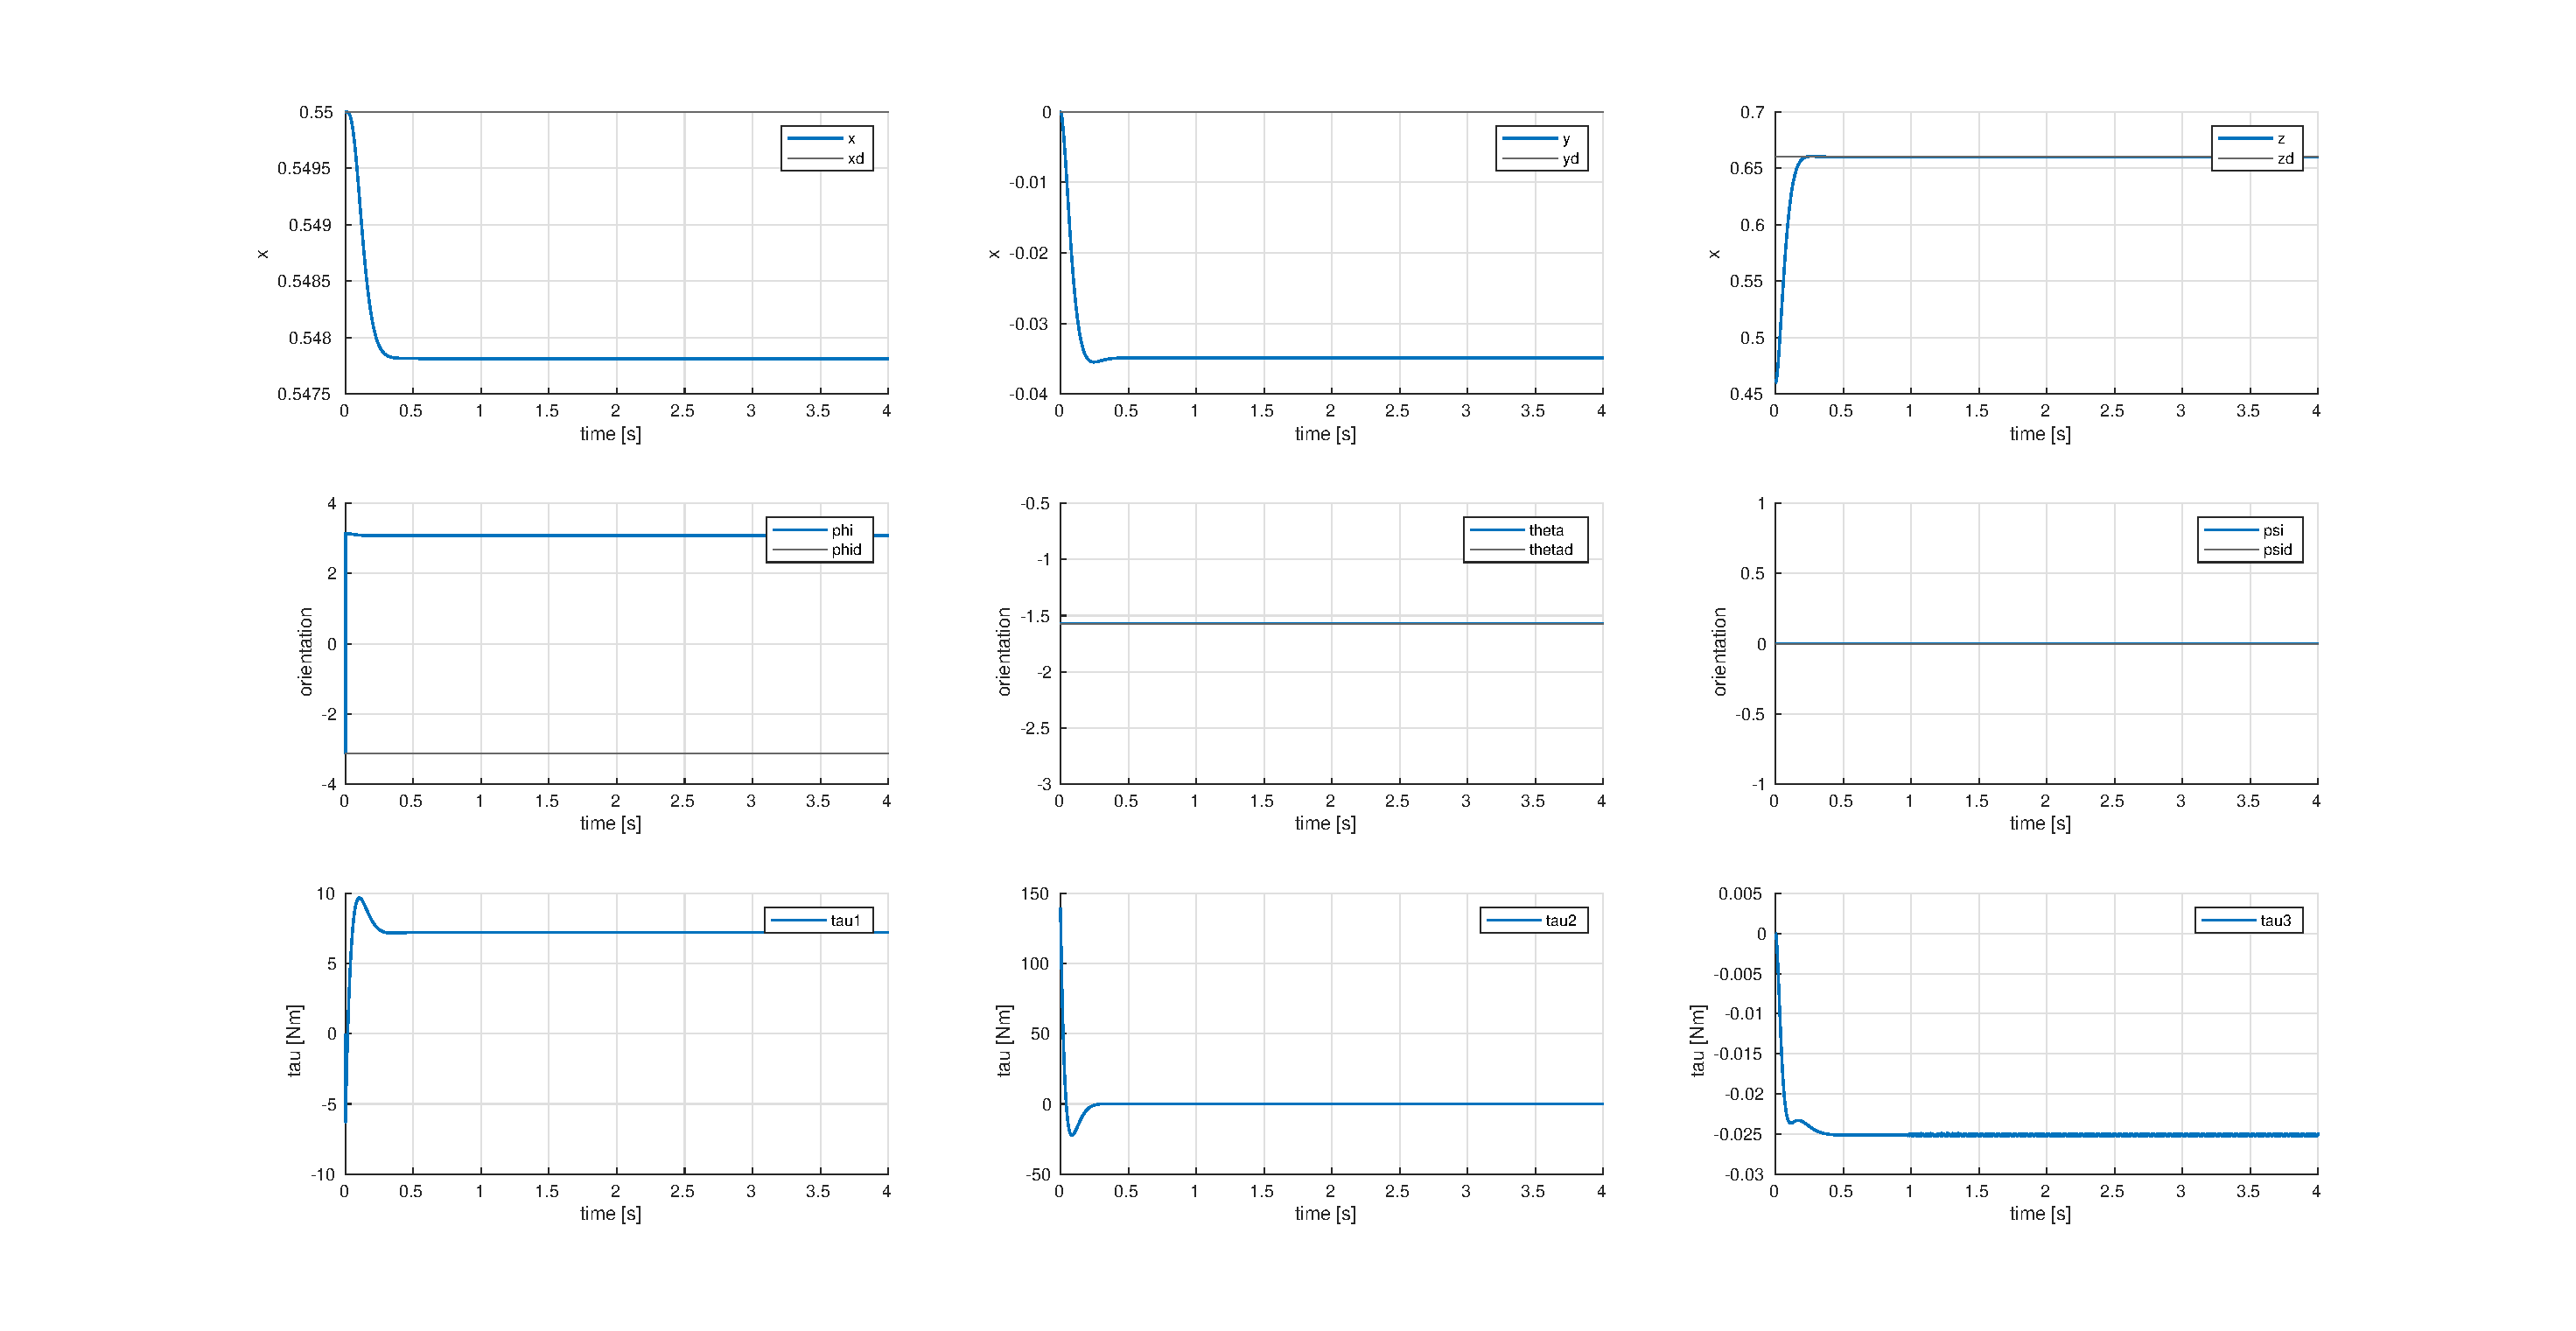
\includegraphics[scale=0.5]{images/op_without_gravity.eps}
    \end{center}
    \caption{Operational Space PD control without graviy compensation}
    \label{fig:without_gravity_op}
\end{figure}

\newpage
\subsection{Operational Space Inverse Dynamic PD control}

The operational space inverse dynamics PD control architecture was introduced to solve the tracking problem using the 3DOF manipulator. In Fig \ref{fig:op_inv_dyn} an example of the response obtained using a polynomial trajectory. The waypoints provided are $ q = [0,2,3;1,3,1;0,1,1] $ at time $t = [ 0, 2, 4 ] $
\begin{figure}[H]
    \begin{center}
        \hspace*{-4.5cm}
        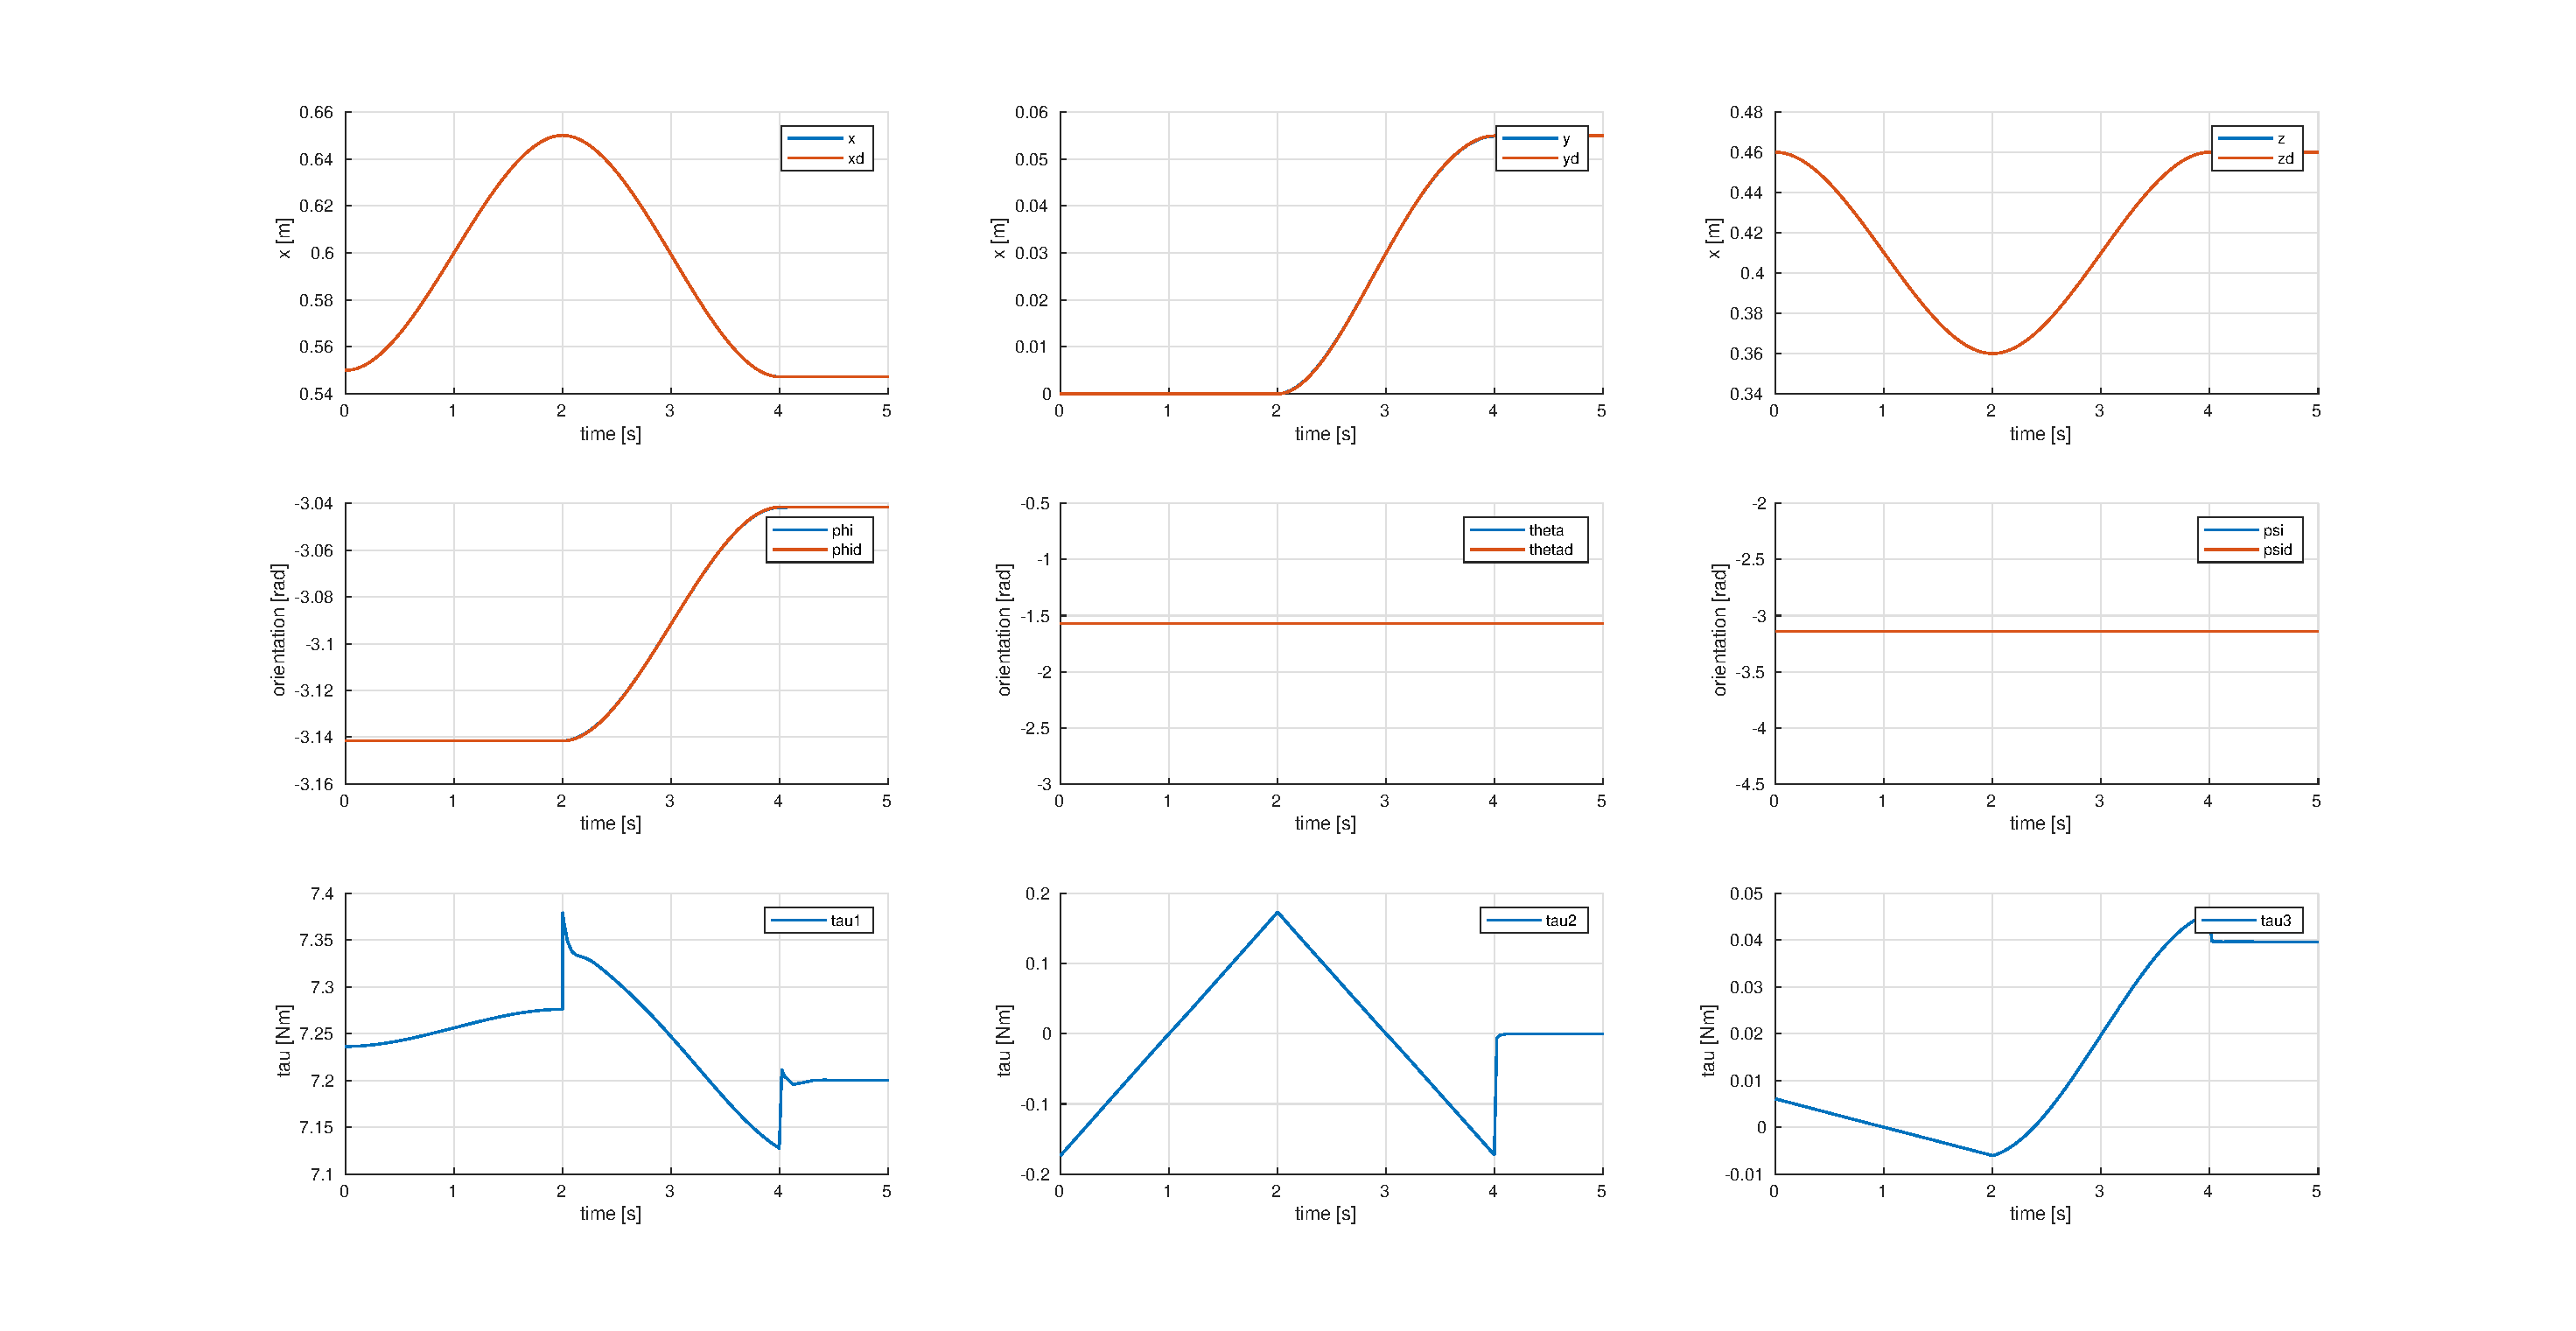
\includegraphics[scale=0.5]{images/op_inv_dyn.eps}
    \end{center}
    \caption{Operational Space Inverse dynamic PD control}
    \label{fig:op_inv_dyn}
\end{figure}


\end{document}